% =============================================================
% Presentación de Trabajo de Grado · INMU / Índice Urbano Global
% Pontificia Universidad Javeriana · 2026
%
% Compilación recomendada:
%   En Overleaf: compilador pdfLaTeX (configuración por defecto).
%
% Estructura:
%   - Beamer con tema metropolis (debería estar pre-instalado en Overleaf).
%   - Bibliografía manual con thebibliography (no usa .bib externo).
%   - Slots para gráficas vía \figslot{descripción}{ruta}; si el PDF
%     existe en figs/ se inserta, si no, muestra un placeholder.
%
% Carpetas esperadas:
%   figs/    ← coloca aquí tus gráficas hechas a mano (PNG/PDF).
% =============================================================
\documentclass[aspectratio=169,11pt]{beamer}

% ---- Paquetes esenciales ---------------------------------------
\usepackage[utf8]{inputenc}
\usepackage[spanish]{babel}
\usepackage[T1]{fontenc}
\usepackage{lmodern}
\usepackage{amsmath, amssymb}
\usepackage{booktabs, array}
\usepackage{graphicx}
\usepackage{grffile}  % permite espacios y múltiples puntos en nombres de archivo
\usepackage{tikz}
\usetikzlibrary{positioning, arrows.meta, calc, shapes.geometric, shapes.symbols}
% shapes.geometric → diamond (decisión en el pipeline RAG)
% shapes.symbols   → cylinder (stores de datos: Gemini, OSM, PostGIS, Redis)
% calc             → ($(a)!t!(b)$) para posicionar etiquetas en spokes del pentágono
\usepackage{xcolor}
\usepackage{multicol}
\usepackage{hyperref}
\usepackage{appendixnumberbeamer}
% NOTA: NO usar biblatex aquí. Usamos thebibliography clásico con \cite{...}.
%       Si más adelante migras a .bib, reemplaza la sección de Referencias
%       por \printbibliography y carga \usepackage{biblatex} + \addbibresource.

% ---- Tema y paleta INMU ----------------------------------------
\usetheme{metropolis}
\usecolortheme{default}

\definecolor{inmuPrimary}{HTML}{0A2540}
\definecolor{inmuGreen}{HTML}{15803D}
\definecolor{inmuGreenLight}{HTML}{22C55E}
\definecolor{inmuBlue}{HTML}{2563EB}
\definecolor{inmuBlueLight}{HTML}{60A5FA}
\definecolor{inmuSurface}{HTML}{F8FAFC}
\definecolor{inmuMuted}{HTML}{64748B}
\definecolor{dockerBlue}{HTML}{2496ED}

\setbeamercolor{normal text}{fg=inmuPrimary, bg=white}
\setbeamercolor{frametitle}{fg=white, bg=inmuPrimary}
\setbeamercolor{title}{fg=inmuPrimary}
\setbeamercolor{author}{fg=inmuMuted}
\setbeamercolor{date}{fg=inmuMuted}
\setbeamercolor{alerted text}{fg=inmuGreen}
\setbeamercolor{block title}{fg=white, bg=inmuGreen}
\setbeamercolor{block body}{fg=inmuPrimary, bg=inmuSurface}
% Alertblock: por defecto metropolis usa `alerted text` como fg del título,
% y al ser inmuGreen sobre fondo verde queda invisible. Lo forzamos a
% blanco sobre verde para que se lea igual que los `block` normales.
\setbeamercolor{block title alerted}{fg=white, bg=inmuGreen}
\setbeamercolor{block body alerted}{fg=inmuPrimary, bg=inmuSurface}
\setbeamercolor{itemize item}{fg=inmuGreen}
\setbeamercolor{itemize subitem}{fg=inmuGreen}

\metroset{progressbar=frametitle, sectionpage=progressbar}

% ====================================================================
% NOTAS DEL EXPOSITOR
% --------------------------------------------------------------------
%  Cada frame tiene un \note{...} con las CITAS exactas + puntos clave
%  para sustentación. Por defecto las notas NO se ven en el PDF de los
%  slides (queda limpio para proyectar). Para verlas, descomenta UNA
%  de las siguientes opciones según el modo que necesites:
%
%   - Solo slides limpios (DEFAULT — para sustentar):
%     ↓ no descomentes nada
%
%   - Slides + notas en páginas alternadas (para imprimir):
%     \setbeameroption{show notes}
%
%   - PDF widescreen con slide a la izquierda + nota a la derecha
%     (ideal para abrir en el laptop mientras proyecta el slide):
%     \setbeameroption{show notes on second screen=right}
%
%   - Solo notas (sin slides):
%     \setbeameroption{show only notes}
% ====================================================================
\setbeamertemplate{note page}{%
  \insertnote
}

% ---- Metadatos -------------------------------------------------
\title{Índice Urbano Global de Bogotá (IUG)}
\subtitle{Mide la calidad urbana antes de mirar el precio}
\author{Neyl Peñuela Bernate \\ \small Director: Vladimir Moreno G.}
\institute{Pontificia Universidad Javeriana \\ Programa de Ciencia de Datos}
\date{Sustentación · Mayo 2026}

% ---- Helpers ---------------------------------------------------
% IMPORTANTE: \dim ya está reservado en LaTeX (operador matemático),
%             usamos \hi (highlight) y \hl (highlight-light) en su lugar.
\newcommand{\hi}[1]{\textcolor{inmuGreen}{\textbf{#1}}}
\newcommand{\hl}[1]{\textcolor{inmuGreen}{#1}}

% Slot para gráfico: si compilas con \includegraphics y el archivo no
% existe, pdfLaTeX falla. Por eso usamos un placeholder visible — basta
% reemplazarlo manualmente por \includegraphics cuando tengas la figura.
\newcommand{\figslot}[2]{%
  \begin{center}
    \fbox{\begin{minipage}{0.85\linewidth}\centering
      \vspace{2em}\textit{[ Aquí va: #1 ]}\\\small\texttt{\detokenize{#2}}\vspace{2em}
    \end{minipage}}
  \end{center}
}

% Nota al pie del slide con citas — se ancla abajo a la izquierda en
% gris suave. Se usa al final del frame y enumera las referencias clave
% que sustentan la metodología expuesta arriba.
\newcommand{\framenote}[1]{%
  \vfill
  {\scriptsize\color{inmuMuted}\textbf{Fundamento metodológico:}\ #1}%
}

\begin{document}

% ================================================================
% Portada
% ================================================================
\begin{frame}[plain]
  \titlepage
\end{frame}

% ================================================================
% SECCIÓN 1: INTRODUCCIÓN Y POSICIONAMIENTO
% ================================================================
\section{Introducción}

\begin{frame}{Motivación: La asimetría en el mercado}
  \begin{columns}[T,onlytextwidth]
    \column{0.55\textwidth}
      \begin{itemize}
        \item El valor de mercado es una \hl{mezcla heterogénea}: atributos físicos, inercia histórica y percepciones subjetivas.
        \item \hi{Problema:} El precio suele estar desconectado de los fundamentales urbanos (seguridad real, dotación, normativa).
        \item Existe una \hi{asimetría de información} entre el inversor/comprador y la realidad del territorio.
      \end{itemize}
    \column{0.42\textwidth}
      % Scatter ilustrativo Precio vs Calidad: si el mercado fuera eficiente,
      % todos los puntos caerían sobre la diagonal. La dispersión a lado y
      % lado de la diagonal ES la asimetría que motiva el IUG.
      \begin{center}
      \begin{tikzpicture}[font=\scriptsize, scale=0.95]
        % Marco
        \draw[draw=inmuMuted, thick] (0,0) rectangle (5.2,4.2);
        % Ejes (dentro del marco)
        \draw[->, color=inmuPrimary, thick] (0.5,0.5) -- (5.0,0.5)
          node[below right, font=\scriptsize, text=inmuPrimary] {Precio};
        \draw[->, color=inmuPrimary, thick] (0.5,0.5) -- (0.5,4.0)
          node[above left, rotate=90, anchor=south west, font=\scriptsize, text=inmuPrimary] {Calidad urbana};
        % Diagonal "mercado eficiente"
        \draw[dashed, color=inmuMuted, thick] (0.5,0.5) -- (4.8,3.8)
          node[midway, sloped, above, font=\tiny, text=inmuMuted] {mercado eficiente};
        % Nube de puntos lejos de la diagonal (asimetría) — verdes en cuadrantes "buy/sell"
        % Cuadrante "COMPRAR": calidad alta, precio bajo (arriba-izquierda)
        \fill[inmuGreen] (1.3,3.0) circle (3pt);
        \fill[inmuGreen] (1.6,3.4) circle (3pt);
        \fill[inmuGreen] (1.9,2.8) circle (3pt);
        \fill[inmuGreen] (1.1,2.4) circle (3pt);
        \fill[inmuGreen] (2.2,3.2) circle (3pt);
        \node[text=inmuGreen, font=\tiny\bfseries, rotate=10] at (1.4,3.7) {COMPRAR};
        % Cuadrante "VENDER": calidad baja, precio alto (abajo-derecha)
        \fill[red!75!black] (3.6,1.0) circle (3pt);
        \fill[red!75!black] (4.0,1.4) circle (3pt);
        \fill[red!75!black] (4.3,0.9) circle (3pt);
        \fill[red!75!black] (3.3,1.3) circle (3pt);
        \fill[red!75!black] (4.5,1.6) circle (3pt);
        \node[text=red!75!black, font=\tiny\bfseries, rotate=-10] at (4.0,0.7) {VENDER};
        % Puntos sobre la diagonal (mercado coherente, gris)
        \fill[inmuMuted!70] (2.5,2.3) circle (2pt);
        \fill[inmuMuted!70] (3.0,2.7) circle (2pt);
        \fill[inmuMuted!70] (3.5,3.1) circle (2pt);
        \fill[inmuMuted!70] (2.0,1.8) circle (2pt);
        \fill[inmuMuted!70] (1.5,1.4) circle (2pt);
      \end{tikzpicture}
      \\[0.2em]
      {\tiny\itshape Cada punto = un inmueble. Distancia a la diagonal = magnitud de la asimetría.}
      \end{center}
  \end{columns}
  \framenote{Exuberancia irracional~\cite{shiller2015}; composición del precio hedónico~\cite{rosen1974}.}
\end{frame}

\begin{frame}{Posicionamiento: IUG $\neq$ Predictor de Precio}
  \begin{columns}[T,onlytextwidth]
    \column{0.48\textwidth}
      \begin{block}{Modelos AVM (Lo que ya existe)}
        \small
        Familias maduras de \textit{Automated Valuation Models} cuyo fin es \hi{predecir el precio}.
        \begin{itemize}
          \item Métricas \textbf{IAAO} establecidas.
          \item Indicadores de calidad: \textbf{COD, PRD, PRB}.
          \item Foco en precisión estadística sobre el valor transaccional.
        \end{itemize}
      \end{block}
    \column{0.48\textwidth}
      \begin{alertblock}{El IUG (Propuesta)}
        \small
        Una \hi{herramienta-perspectiva}: instrumento analítico que no busca inferir el precio.
        \begin{itemize}
          \item Condensa \textbf{5 metodologías heterogéneas}.
          \item Foco en la \textbf{ortogonalidad}: medir lo que el precio no captura.
          \item Revelar la brecha entre mercado y entorno objetivo.
        \end{itemize}
      \end{alertblock}
  \end{columns}
  \note{\scriptsize
    Es vital dejar claro al jurado que NO estamos compitiendo con un AVM. 
    Mencionar métricas IAAO (Standard on Ratio Studies) demuestra dominio del estado del arte. 
    El IUG es complementario: el AVM dice cuánto cuesta, el IUG dice qué tan bueno es el entorno.
  }
\end{frame}

\begin{frame}{Delimitación Legal y Técnica}
  \begin{itemize}
    \item \textbf{Complemento, no sustitución:} El IUG ofrece un \hi{complemento analítico} para la toma de decisiones, no una base regulatoria.
    \item \textbf{Marco Normativo:} No constituye instrumento tributario ni base catastral oficial bajo la \hi{Resolución IGAC 1912 de 2024}.
    \item \textbf{Independencia:} Al ser calculado con fuentes abiertas (IDECA, SDP, DANE), el indicador se mantiene libre de los sesgos de la oferta inmobiliaria.
  \end{itemize}
  \begin{exampleblock}{Veredicto Metodológico}
    La débil correlación con el precio no es un error del modelo, es la \textbf{prueba de su utilidad informativa}.
  \end{exampleblock}
  \framenote{Resolución IGAC 1912 de 2024~\cite{IGAC1912}; postura metodológica del IUG (Capítulo 1.3.1 de la tesis).}
\end{frame}
% ================================================================
% SECCIÓN 2: OBJETIVOS
% ================================================================

\begin{frame}{Objetivo General}
  \begin{block}{Declaración central}
    Diseñar, implementar y validar el \hi{Índice Urbano Global (IUG)} como una herramienta poblacional, abierta y reproducible que sintetice cinco dimensiones del bienestar urbano de Bogotá en una métrica única, independiente del precio de mercado, y que opere como sistema de soporte a la decisión inmobiliaria.
  \end{block}
  \vspace{1em}
  \begin{itemize}
    \item \textbf{No es:} Un estimador de precios predictivo.
    \item \textbf{Sí es:} Un sistema de soporte a la decisión basado en las calidades del entorno.
  \end{itemize}
\end{frame}
\note{\scriptsize
  \textbf{Discurso:}
  El objetivo general es la columna vertebral de la tesis. Aquí se debe hacer énfasis en tres palabras clave: **Poblacional** (porque abarca toda la oferta, no solo una muestra pequeña), **Abierta** (porque usa datos oficiales) e **Independiente** (porque no se contamina con el precio observado).
}

\begin{frame}{Objetivos Específicos (1/2): Construcción y Modelado}
  \begin{enumerate}
    \item \textbf{Operacionalizar dimensiones:} Transformar cinco dimensiones del entorno urbano (accesibilidad, seguridad, calidad construida, dotación y potencial normativo) en subíndices comparables usando datos oficiales (DANE, IDECA, SDP, POT 555, EPV 2024, ICSU).
    \item \textbf{Pipeline de datos reproducible:} Construir una arquitectura que integre extracción automatizada, asignación espacial PostGIS y control de calidad con DBSCAN, garantizando la trazabilidad desde el anuncio hasta el indicador.
    \item \textbf{Benchmark hedónico:} Estimar un modelo de referencia (OLS, Ridge, Lasso, Elastic Net) no para predecir, sino para usarlo como línea base y contrastar la información incremental que aporta el IUG.
  \end{enumerate}
\end{frame}

\begin{frame}{Objetivos Específicos (2/2): Validación y Producto}
  \begin{enumerate}
    \setcounter{enumi}{3} % Continúa la numeración desde el 4
    \item \textbf{Validación estadística:} Ejecutar un protocolo de 11 pruebas (incluyendo bootstrap, modelos anidados, comunalidad, Ramsey RESET y validación cruzada espacial) para garantizar la robustez y validez de uso.
    \item \textbf{Cuantificación de incertidumbre:} Analizar la varianza y sensibilidad del indicador (índices de Sobol/Saltelli) ante perturbaciones en los pesos metodológicos.
    \item \textbf{Despliegue operativo:} Habilitar el acceso al sistema mediante una plataforma web y un asistente conversacional (arquitectura RAG), democratizando el análisis sin requerir conocimientos en geoestadística.
  \end{enumerate}
\end{frame}
\note{\scriptsize
  \textbf{Discurso:}
  \begin{itemize}\itemsep0pt
    \item Dividir los objetivos ayuda a la audiencia a respirar.
    \item Los primeros 3 son de **Ingeniería y Economía** (construir el dato y el baseline).
    \item Los últimos 3 son de **Ciencia de Datos y Producto** (validar que el dato es bueno y ponérselo en las manos al usuario con RAG).
  \end{itemize}
}

% ================================================================
% SECCIÓN 2: MARCO TEÓRICO Y "REGLAS DE JUEGO"
% ================================================================
\section{Marco teórico y conceptual}

\begin{frame}{Las Reglas de Juego: Conceptos Transversales}
  \begin{columns}[T,onlytextwidth]
    \column{0.5\textwidth}
      \textbf{1. Primera Ley de Tobler (1970)}
      \begin{itemize}
        \item \textit{``Todo está relacionado, pero lo cercano está más relacionado.''}\\[0.2em]
        \footnotesize \hi{Aplicación:} Justifica medir distancias y usar áreas de influencia espaciales en la ciudad.
      \end{itemize}
      
      \vspace{0.6em}
      \textbf{2. Autocorrelación e Índice de Moran}
      \begin{itemize}
        \item Mide si valores similares tienden a agruparse en el espacio (clústers) o si son aleatorios.\\[0.2em]
        \footnotesize \hi{Aplicación:} Evaluar la estabilidad espacial y el ``contagio'' de precios entre barrios.
      \end{itemize}

    \column{0.5\textwidth}
      \textbf{3. Estandarización vs. Studentización}
      \begin{itemize}
        \item Usamos \textit{Rank Min-Max} $[0,5]$ (estandarizado) en lugar de \textit{Z-scores} (studentizado).
        \item \textbf{¿Por qué?} La calidad urbana tiene límites físicos finitos (ej. distancia cero a un parque), no colas infinitas. Evita penalizar distribuciones asimétricas naturales.
      \end{itemize}

      \vspace{0.6em}
      \textbf{4. Correlación y Ortogonalidad}
      \begin{itemize}
        \item La independencia estadística ($r \approx 0$) indica que dos métricas cuentan historias diferentes.
      \end{itemize}
  \end{columns}
  \framenote{Primera ley de la geografía~\cite{tobler1970}; Índice de Moran y LISA~\cite{anselin1995}.}
\end{frame}
\note{\scriptsize
  \textbf{Discurso:}
  Antes de armar el indicador, estas son las cuatro reglas del juego. 
  Hacer énfasis en el punto 3 (Min-Max vs Z-Score): Si usamos Z-score (studentizar), asumimos medias centradas y normalidad. Ya probamos que en el mundo inmobiliario los datos son bimodales o asimétricos. El Min-Max respeta esa forma original y pone a todos a competir en una cancha fija de 0 a 5.
}

\begin{frame}{Caja de Herramientas: Conectando concepto con dimensión}
  Cada subíndice del IUG aplica un concepto geoestadístico específico para resolver su medición:

  \vspace{0.6em}
  \begin{description}[Modelo Gravitacional] % Ajusta la sangría
    \item[Modelo Gravitacional $\to$ I\_ACC:] Basado en el concepto de \emph{masa potencial}. No solo mide ``qué tan cerca'' está el transporte, sino cuánto ``pesa'' esa estación (su capacidad) descontada por la fricción de la distancia.
    \item[Proximidad Acumulada $\to$ I\_DOT:] Sumatoria espacial de Puntos de Interés (POIs). Aplica \emph{buffers caminables} (400m y 800m) donde el acceso inmediato vale más.
    \item[Score con PCA $\to$ I\_HED:] \emph{Análisis de Componentes Principales}. Comprime atributos multicolineales (área, baños, garajes) internos del inmueble en un único vector de varianza latente (confort privado).
  \end{description}
  
  \vspace{0.6em}
  \begin{center}
    \footnotesize \hi{Hilo conductor:} Juntar estas metodologías heterogéneas requiere unificarlas bajo la estandarización $[0,5]$ mencionada anteriormente.
  \end{center}
\end{frame}
\note{\scriptsize
  \textbf{Discurso:}
  Aquí conectamos el diccionario con el indicador. El IUG no es una simple suma matemática; es un ensamble de modelos.
  - El transporte funciona con gravedad (fricción de distancia).
  - Los parques y colegios funcionan con proximidad peatonal (buffers).
  - El inmueble por dentro funciona con reducción de dimensionalidad (PCA).
}

\begin{frame}{Paradigma Econométrico: Validar por Adición, no por Ajuste}
  \begin{block}{El uso de la Regresión Lineal Múltiple}
    \small
    En este trabajo, la econometría no se usa para predecir precios. Se usa para demostrar \hi{adición de información}. Si agregamos el IUG a un modelo base y el $\Delta R^2$ sube significativamente, comprobamos que el indicador porta valor oculto.
  \end{block}

  \vspace{0.5em}
  \textbf{La validación empírica se establece por 4 propiedades verificables:}
  \begin{enumerate}
    \item \hi{Ortogonalidad informativa:} El IUG correlaciona débilmente con el precio; captura la calidad de vida que el mercado ignora.
    \item \hi{Robustez ante perturbaciones:} Los scores no colapsan frente a valores atípicos espaciales o cambios de muestra.
    \item \hi{Estabilidad espacial:} Controla el sesgo regional (demostrado con Índice de Moran sobre los residuos).
    \item \hi{Capacidad de discriminar segmentos:} Puede partir el mercado en agrupaciones accionables estadísticamente distintas.
  \end{enumerate}
  \framenote{Desplazamiento del enfoque predictivo al inferencial~\cite{nimon2013}; análisis de varianza común para descomponer R$^2$.}
\end{frame}
\note{\scriptsize
  \textbf{Discurso:}
  Esta diapositiva es el ``jaque mate'' metodológico. 
  Si el jurado pregunta por qué la regresión no tiene un R2 de 0.90, esta es la respuesta: ``No quiero un R2 alto. Quiero demostrar que la regresión base de atributos tiene un R2 de X, y cuando le meto el IUG sube a X + Delta. Ese Delta es el valor incremental. Lo valido probando que es ortogonal, robusto, espacialmente estable y que sirve para encontrar mispricing (segmentar el mercado)''.
}

% ================================================================
\section{Metodología · CRISP-DM y las 5 dimensiones}
% ================================================================

\begin{frame}{Estructura General del IUG}
  \[
    \mathrm{IUG}_i \;=\; w_{\text{acc}} \, I_{\text{ACC},i}
                  \,+\, w_{\text{seg}} \, I_{\text{SEG},i}
                  \,+\, w_{\text{hed}} \, I_{\text{HED},i}
                  \,+\, w_{\text{dot}} \, I_{\text{DOT},i}
                  \,+\, w_{\text{pnu}} \, I_{\text{PNU},i}
  \]
  \begin{center}
    \footnotesize Cada subíndice $I_{\bullet,i} \in [0, 5]$ tras
    \textit{rank min-max} y pesos equiponderados por defecto (0.20 c/u).
  \end{center}
  \vspace{0.4em}
  \begin{block}{Premisa de Independencia}
    Los datos de entrada son \emph{independientes} de la oferta inmobiliaria (DANE, IDECA, SDP, EPV 2024, POT 555, IDRD). Esto es el núcleo para garantizar la \hi{ortogonalidad al precio}.
  \end{block}
  \framenote{Equiponderación [0.20 c/u] recomendada por OECD ante falta de priorización a priori~\cite{nardo2008}.}
\end{frame}
\note{\scriptsize
\textbf{Discurso:}
\begin{itemize}\itemsep0pt
  \item Presentamos el IUG como una agregación lineal compensatoria (una zona puede compensar baja accesibilidad con buena dotación).
  \item Datos abiertos = replicabilidad.
\end{itemize}
}

% ================================================================
% NUEVO FRAME: PENTÁGONO DE LOS 5 SUBÍNDICES (TikZ)
% ================================================================
\begin{frame}{Las cinco dimensiones del IUG}
  \begin{center}
    \resizebox{!}{0.78\textheight}{%
    \begin{tikzpicture}[
        font=\small,
        % Estilos
        vertex/.style={
          rectangle, rounded corners=6pt,
          draw=inmuPrimary, line width=1pt,
          fill=inmuSurface, align=center,
          inner sep=6pt, minimum width=3.6cm, minimum height=2.2cm
        },
        core/.style={
          circle, draw=inmuGreen, line width=1.5pt,
          fill=inmuGreen!10, align=center,
          minimum size=2.6cm
        },
        spoke/.style={->, >=latex, thick, color=inmuPrimary, opacity=0.55},
        ring/.style={dashed, draw=inmuMuted, opacity=0.55, thick},
        iconlabel/.style={font=\scriptsize\bfseries, text=inmuPrimary},
        sublabel/.style={font=\tiny, text=inmuMuted}
      ]

      % Radio del pentágono (centro -> vértice)
      \def\R{5.4}

      % --- IUG en el centro ---
      \node[core] (iug) at (0,0) {
        \textbf{\large IUG}\\
        \scriptsize PCA\\
        \scriptsize 5 dim
      };

      % --- 5 vértices del pentágono (top, UL, LL, LR, UR) ---
      % Ángulos: 90, 162, 234, 306, 18 (regular, vértice arriba)
      \node[vertex] (acc) at ({90}:\R)  {
        
\includegraphics[height=1.1cm]{figs/icons/bus-stop.png}\\[2pt]
        \textbf{\textcolor{inmuPrimary}{I\_ACC}}\\
        \scriptsize Accesibilidad\\
        \tiny TransMilenio · SITP
      };
      \node[vertex] (seg) at ({162}:\R) {
        
\includegraphics[height=1.1cm]{figs/icons/cyber-security.png}\\[2pt]
        \textbf{\textcolor{inmuPrimary}{I\_SEG}}\\
        \scriptsize Seguridad\\
        \tiny EPV 2024 · ICSU · CAI
      };
      \node[vertex] (hed) at ({234}:\R) {
        
\includegraphics[height=1.1cm]{figs/icons/balance.png}\\[2pt]
        \textbf{\textcolor{inmuPrimary}{I\_HED}}\\
        \scriptsize Hedónico\\
        \tiny PCA · KNN espacial
      };
      \node[vertex] (dot) at ({306}:\R) {
        
\includegraphics[height=1.1cm]{figs/icons/cityscape.png}\\[2pt]
        \textbf{\textcolor{inmuPrimary}{I\_DOT}}\\
        \scriptsize Dotación\\
        \tiny Salud · Educación · Parques
      };
      \node[vertex] (pnu) at ({18}:\R)  {
        
\includegraphics[height=1.1cm]{figs/icons/construction-site.png}\\[2pt]
        \textbf{\textcolor{inmuPrimary}{I\_PNU}}\\
        \scriptsize Potencial normativo\\
        \tiny POT 555 · SDP
      };

      % --- Anillo pentagonal entre vértices (sutil) ---
      \draw[ring] (acc) -- (seg) -- (hed) -- (dot) -- (pnu) -- cycle;

      % --- Spokes (centro -> vértice) con peso 0.20 ---
      \foreach \v in {acc, seg, hed, dot, pnu} {
        \draw[spoke] (iug) -- (\v);
      }

      % --- Pesos sobre las flechas ---
      \node[sublabel, fill=white, inner sep=1pt] at ($(iug)!0.55!(acc)$) {$w=0.20$};
      \node[sublabel, fill=white, inner sep=1pt] at ($(iug)!0.55!(seg)$) {$w=0.20$};
      \node[sublabel, fill=white, inner sep=1pt] at ($(iug)!0.55!(hed)$) {$w=0.20$};
      \node[sublabel, fill=white, inner sep=1pt] at ($(iug)!0.55!(dot)$) {$w=0.20$};
      \node[sublabel, fill=white, inner sep=1pt] at ($(iug)!0.55!(pnu)$) {$w=0.20$};

    \end{tikzpicture}%
    }
  \end{center}
  \vspace{-0.6em}
  \framenote{Pentágono balanceado por defecto (\textit{equiponderación}); pesos ajustables vía AHP~\cite{saaty1980,ishizaka2011} para perfiles de usuario.}
\end{frame}
\note{\scriptsize
\textbf{Discurso:}
\begin{itemize}\itemsep0pt
  \item Cada vértice es una dimensión independiente del precio: medimos calidad urbana \emph{antes} de mirar el valor de mercado.
  \item Las 5 contribuyen al núcleo (IUG) por PCA. La equiponderación 0.20 es el caso base; AHP permite que un usuario priorice (p.ej. familia con niños sube I\_SEG e I\_DOT).
  \item El anillo entre vértices sugiere que las dimensiones interactúan pero no se solapan (ortogonalidad ≈ 0).
\end{itemize}
}

% ================================================================
% NUEVO FRAME: CRISP-DM (Diagrama)
% ================================================================
\begin{frame}{Marco de Trabajo: Metodología CRISP-DM}
  \begin{center}
    % Usamos 0.95\textheight o \linewidth para asegurar que no se desborde
    \resizebox{!}{0.75\textheight}{%
    \begin{tikzpicture}[
        node distance=0.8cm and 1.2cm,
        font=\footnotesize,
        % Estilos de los nodos adaptados a la paleta INMU
        phase/.style={
            rectangle,
            draw=inmuPrimary,
            fill=inmuSurface,
            rounded corners,
            minimum width=4.5cm,
            minimum height=2cm,
            align=left,
            line width=0.8pt
        },
        % Estilos de las flechas
        arrow/.style={->, >=latex, very thick, color=inmuPrimary},
        cyclearrow/.style={->, >=latex, thick, dashed, color=inmuGreen}
    ]

    % -- Fila Superior --
    \node[phase] (bu) {\textbf{\textcolor{inmuPrimary}{1. Business Understanding}}\\$\bullet$ Objetivo: IUG vs. Precio\\$\bullet$ KPI: Ratio Oportunidad\\$\bullet$ Alcance: Bogotá};

    \node[phase, right=of bu] (du) {\textbf{\textcolor{inmuPrimary}{2. Data Understanding}}\\$\bullet$ Exploración de Portales\\$\bullet$ Calidad (IGAC/SIEDCO)\\$\bullet$ Cobertura Espacial};

    % -- Fila Central --
    \node[phase, below=of du] (dp) {\textbf{\textcolor{inmuPrimary}{3. Data Preparation}}\\$\bullet$ ETL Distribuido\\$\bullet$ Geocodificación\\$\bullet$ Snapping Espacial};

    \node[phase, left=of dp] (mo) {\textbf{\textcolor{inmuPrimary}{4. Modeling}}\\$\bullet$ Modelos base y IUG\\$\bullet$ PCA y AHP\\$\bullet$ Regresión espacial};

    % -- Fila Inferior --
    \node[phase, below=of mo] (ev) {\textbf{\textcolor{inmuPrimary}{5. Evaluation}}\\$\bullet$ Pruebas ortogonalidad\\$\bullet$ Robustez (Bootstrap)\\$\bullet$ Segmentación de mercado};

    \node[phase, right=of ev] (de) {\textbf{\textcolor{inmuPrimary}{6. Deployment}}\\$\bullet$ API FastAPI / pgvector\\$\bullet$ Asistente RAG\\$\bullet$ Mapas Interactivos};

    % -- Conexiones de Flujo (Camino Feliz en forma de S) --
    \draw[arrow] (bu) -- (du);
    \draw[arrow] (du) -- (dp);
    \draw[arrow] (dp) -- (mo);
    \draw[arrow] (mo) -- (ev);
    \draw[arrow] (ev) -- (de);

    % -- Retroalimentaciones (Ciclos Iterativos) --
    % De Evaluación a Entendimiento del Negocio (bend left largo)
    \draw[cyclearrow, bend left=45] (ev.west) to node[left, font=\scriptsize, text=inmuMuted, align=right]{Refinar\\Objetivos} (bu.west);

    % De Modelado a Preparación de Datos (flecha recta sobre ellos)
    \draw[cyclearrow, transform canvas={yshift=0.2cm}] (mo.east) -- node[above, font=\scriptsize, text=inmuMuted]{Ajuste ETL} (dp.west);

    \end{tikzpicture}%
    }
  \end{center}
  \vspace{-1em} % Compensa un poco el margen inferior
  \framenote{El flujo iterativo de CRISP-DM soporta la trazabilidad desde la ingesta de datos hasta la plataforma operativa.}
\end{frame}
\note{\scriptsize
  \textbf{Discurso:}
  \begin{itemize}\itemsep0pt
    \item Presentar este mapa mental demuestra que el IUG no es un análisis aislado, sino el núcleo de un producto de datos iterativo.
    \item Mostrar cómo el proyecto fluye en forma de ``S'': empezamos entendiendo el problema de la asimetría (1), auditamos datos oficiales (2 y 3), construimos el IUG (4, foco de la presentación), lo validamos econométricamente (5) y lo disponibilizamos en una plataforma (6).
    \item Las flechas punteadas verdes muestran que si el modelo falla en su validación cruzada, nos obliga a repensar las variables (Ajuste ETL) o el alcance del negocio.
  \end{itemize}
}

% ================================================================
% NUEVO FRAME: REPRODUCIBILIDAD CON DOCKER
% ----------------------------------------------------------------
% Refuerza la fase 6 de CRISP-DM (Deployment) y conecta con
% Arquitectura. Logo opcional en figs/docker.png; si no existe se
% dibuja un placeholder TikZ con la ballena/contenedores.
% ================================================================
\begin{frame}{Reproducibilidad · todo el stack en \texttt{docker compose up}}
  % Logo oficial de Docker (pequeño) en la esquina inferior-derecha del frame.
  % Overlay sin afectar el layout de las columnas.
  \IfFileExists{figs/docker.pdf}{%
    \begin{tikzpicture}[remember picture, overlay]
      \node[anchor=south east, xshift=-0.5cm, yshift=1.0cm]
        at (current page.south east)
        {
\includegraphics[height=0.9cm]{figs/docker.pdf}};
    \end{tikzpicture}%
  }{}%
  \begin{columns}[T,onlytextwidth]
    \column{0.38\textwidth}
      \begin{center}
        \resizebox{\linewidth}{!}{%
        \begin{tikzpicture}[font=\small,
            container/.style={
              rectangle, rounded corners=2pt,
              draw=dockerBlue, fill=dockerBlue!12,
              minimum width=2.6cm, minimum height=0.55cm,
              text=inmuPrimary, font=\scriptsize\bfseries
            },
            whale/.style={
              draw=dockerBlue, fill=dockerBlue,
              line width=1pt, rounded corners=4pt
            }
          ]
          % Ballena estilizada de Docker (silueta Moby Dock simplificada).
          % El logo oficial va pequeño en la esquina del frame (overlay
          % fuera del TikZ), no aquí — esto es solo el diagrama del stack.
          \fill[dockerBlue, rounded corners=8pt]
            (-1.6, 3.2) -- (1.6, 3.2) -- (1.6, 2.6) -- (-1.6, 2.6) -- cycle;
          \draw[dockerBlue, line width=1.5pt, rounded corners=4pt]
            (-1.8, 2.6) .. controls (-2.0, 2.4) and (-2.0, 2.2) .. (-1.6, 2.2)
            -- (1.6, 2.2) .. controls (2.0, 2.2) and (2.0, 2.4) .. (1.8, 2.6);
          % Ojo
          \fill[white] (-1.0, 3.0) circle (0.05);
          % Aleta cola
          \fill[dockerBlue] (1.6, 3.2) -- (2.0, 3.5) -- (1.6, 3.0) -- cycle;
          % Contenedores apilados sobre la ballena (servicios reales)
          \node[container] at (0, 1.7) {PostgreSQL 16 + PostGIS};
          \node[container] at (0, 1.05) {pgvector + Redis 7};
          \node[container] at (0, 0.40) {FastAPI + asyncpg};
          \node[container] at (0, -0.25) {React 18 + Vite + Leaflet};
          \node[container, draw=inmuMuted, fill=inmuSurface]
            at (0, -0.95) {Flyway · MongoDB · scrapers};

          % Comando inferior
          \node[anchor=north, font=\ttfamily\scriptsize, text=inmuPrimary]
            at (0, -1.45) {\$ docker compose up -d};
        \end{tikzpicture}%
        }
      \end{center}
    \column{0.58\textwidth}
      \footnotesize
      Un único comando levanta los \hi{7 servicios} del stack con
      versiones congeladas, lo cual transforma INMU en un experimento
      \hi{reproducible bit a bit}:
      \begin{itemize}\itemsep1pt
        \item \hi{Imágenes fijadas} por digest (\texttt{postgis/postgis:16-3.4},
              \texttt{redis:7.2}), sin sorpresas entre máquinas.
        \item \hi{Migraciones versionadas} con Flyway: el esquema
              \texttt{iug.*} se construye igual hoy que en 6 meses.
        \item \hi{Variables y secretos} en \texttt{.env}, fuera del
              repositorio, gobernadas por \texttt{docker-compose} \texttt{secrets}.
        \item \hi{Healthchecks} y orden de arranque
              (\texttt{depends\_on}) explícitos: si PostGIS no responde,
              FastAPI no inicia.
        \item \hi{Volúmenes nombrados} para datos persistentes
              (\texttt{pgdata}, \texttt{redisdata}) — destruibles sin
              tocar el código.
      \end{itemize}
      \vspace{0.3em}
      \begin{center}
        \scriptsize
        \fcolorbox{dockerBlue!50}{dockerBlue!8}{%
          \begin{minipage}{0.95\linewidth}\centering
            \texttt{git clone $\rightarrow$ cp .env.example .env $\rightarrow$ docker compose up}\\[0.2em]
            \scriptsize\itshape\color{inmuMuted}Tres pasos: cualquier jurado puede reproducir el experimento.
          \end{minipage}}
      \end{center}
  \end{columns}
  \framenote{Containerización como condición habilitante de la fase 6 de CRISP-DM (Deployment) y de la reproducibilidad exigida por el método científico.}
\end{frame}
\note{\scriptsize
\textbf{Discurso:}
\begin{itemize}\itemsep0pt
  \item \emph{La reproducibilidad no es un detalle de implementación: es lo que separa un trabajo de grado de un experimento desechable.}
  \item Todo el stack — base espacial, vectorial, caché, API y frontend — corre en contenedores con imágenes y migraciones versionadas. Un \texttt{docker compose up} levanta el sistema completo en cualquier máquina con Docker.
  \item Esto soporta la fase 6 de CRISP-DM (Deployment) y permite que el jurado, o cualquier investigador, replique cifras y mapas sin instalar dependencias localmente.
  \item Si el jurado pregunta por reproducibilidad: ``\emph{el repositorio público + el \texttt{docker-compose.yml} + las migraciones Flyway son suficientes; no hay un paso manual oculto}''.
\end{itemize}
\textbf{Nota técnica:} si \texttt{figs/docker.pdf} o \texttt{figs/docker.png} existe, se usa el logo oficial; si no, se dibuja una silueta TikZ minimalista de Moby Dock.
}

% ================================================================
% NUEVO FRAME: ARQUITECTURA TECNOLÓGICA (TikZ)
% ================================================================
\begin{frame}{Arquitectura de Datos y Plataforma (INMU)}
  \begin{center}
    \resizebox{0.95\linewidth}{!}{%
    \begin{tikzpicture}[
        node distance=0.8cm and 1.2cm,
        font=\small,
        box/.style={
          rectangle, draw=inmuPrimary, fill=inmuSurface,
          rounded corners, minimum width=3.5cm, minimum height=1.5cm,
          align=center, thick
        },
        highlight/.style={box, draw=inmuGreen, fill=inmuSurface},
        edge/.style={->, >=latex, thick, color=inmuPrimary},
        dashedEdge/.style={->, >=latex, thick, dashed, color=inmuMuted}
      ]

      % --- COLUMNA 1: INGESTA ---
      \node[box] (fuentes) {\textbf{Fuentes Oficiales}\\ \scriptsize IDECA, SDP, DANE, IDRD};
      \node[box, below=0.6cm of fuentes] (scraping) {\textbf{Ingesta Scraping}\\ \scriptsize Scrapy · Selenium · Playwright};
      \node[box, below=1cm of scraping] (mongo) {\textbf{Staging DB}\\ \scriptsize MongoDB (raw JSON)};

      \draw[edge] (scraping) -- (mongo);

      % --- COLUMNA 2: CORE DE DATOS (DOCKER) ---
      \node[highlight, right=of scraping, yshift=-0.5cm] (postgis) {\textbf{Motor Espacial}\\ \scriptsize PostgreSQL 16 + PostGIS\\ \scriptsize Flyway (migraciones)};
      \node[box, below=0.6cm of postgis] (pgvector) {\textbf{Motor Vectorial \& Caché}\\ \scriptsize pgvector (RAG)\\ \scriptsize Redis 7};

      \draw[edge] (mongo) -| node[pos=0.25, above, font=\scriptsize, text=inmuPrimary]{ETL · Geocoding} (postgis);
      \draw[edge] (fuentes) -| (postgis);
      \draw[dashedEdge] (postgis) -- (pgvector);

      % --- COLUMNA 3: BACKEND ---
      \node[box, right=of postgis, yshift=-0.5cm] (fastapi) {\textbf{Backend Service}\\ \scriptsize FastAPI + asyncpg\\ \scriptsize JWT · SlowAPI rate-limit};

      \draw[<->, >=latex, thick, color=inmuGreen] (postgis) -- (fastapi);
      \draw[<->, >=latex, thick, color=inmuGreen] (pgvector) -| (fastapi);

      % --- COLUMNA 4: CLIENTE & EDGE ---
      \node[box, right=of fastapi] (react) {\textbf{Aplicación Web}\\ \scriptsize React 18 + Vite\\ \scriptsize Leaflet (mapas 2D)};
      \node[box, above=0.6cm of react] (edgeSec) {\textbf{Edge \& Seguridad}\\ \scriptsize Cloudflare Tunnel\\ \scriptsize Turnstile (captcha)};

      \draw[<->, >=latex, thick, color=inmuPrimary] (fastapi) -- node[above, font=\scriptsize]{REST API} (react);
      \draw[<->, >=latex, thick, color=inmuPrimary] (edgeSec) -- (react);

      % --- MARCO DOCKER ---
      \draw[dashed, draw=inmuMuted, rounded corners, thick]
        ([xshift=-0.4cm, yshift=0.8cm]postgis.north west) rectangle
        ([xshift=0.4cm, yshift=-0.4cm]pgvector.south east);
      \node[text=inmuMuted, font=\scriptsize\bfseries, anchor=south]
        at ([yshift=0.8cm]postgis.north) {Entorno contenerizado (Docker Compose)};

    \end{tikzpicture}%
    }
  \end{center}
  \vspace{-0.8em}
  \framenote{Arquitectura de servicios diseñada para soportar consultas geoespaciales y búsqueda semántica (RAG) en tiempo real.}
\end{frame}
\note{\scriptsize
\textbf{Discurso:}
\begin{itemize}\itemsep0pt
  \item De izquierda a derecha: \emph{ingesta} (scrapers + datos oficiales) → \emph{datos} (PostGIS + pgvector + Redis, todo en Docker) → \emph{backend} (FastAPI async) → \emph{cliente} (React + Leaflet) protegido por Cloudflare Tunnel y Turnstile.
  \item Flechas verdes dobles = comunicación crítica del backend con el motor de datos.
  \item El recuadro punteado encierra los servicios contenerizados, garantizando reproducibilidad mediante \texttt{docker compose up}.
\end{itemize}
}

% ----------------------------------------------------------------
% Frames de los sub-indicadores (con notas corregidas)
% ----------------------------------------------------------------

\begin{frame}{I\_ACC · Accesibilidad (Modelado)}
  \begin{columns}[T,onlytextwidth]
    \column{0.55\textwidth}
      Modelo gravitacional~\cite{hansen1959} sobre TransMilenio + SITP:
      \[
        I_{\text{ACC},i} = \sum_{j \in J} \frac{O_j}{d_{ij}^{\beta}}
      \]
      \begin{itemize}
        \item $O_j$: capacidad/jerarquía de la estación.
        \item $d_{ij}$: distancia geodésica desde el inmueble.
        \item $\beta$: parámetro de decaimiento espacial; calibrado a $\beta \approx 1.5$ siguiendo la metodología de Wilson~\cite{wilson1971} y Fotheringham~\cite{fotheringham1981}.
      \end{itemize}
      \vspace{0.4em}
      Fuentes: TMSA (149 est.), SITP-OSM (7\,693 parad.).
    \column{0.42\textwidth}
      % Histograma inline TikZ — datos reales v2.0 (20 bins de I_ACC)
      \resizebox{\linewidth}{!}{%
      \begin{tikzpicture}[font=\scriptsize]
        % Configuración: 20 bins, x=0..5, alturas proporcionales al conteo
        % Alturas pre-calculadas (h = 4.5 * n / 9212, en cm) para evitar
        % desbordamiento interno de pgfmath con conteos grandes.
        % i=indice del bin (1..20), h=altura ya calculada.
        \foreach \i/\h in {1/4.500, 2/0.137, 3/0.130, 4/0.119, 5/0.166,
                          6/0.194, 7/0.243, 8/0.287, 9/0.380, 10/0.326,
                          11/0.313, 12/0.320, 13/0.381, 14/0.424, 15/0.471,
                          16/0.585, 17/0.842, 18/0.840, 19/0.674, 20/0.277} {
          \pgfmathsetmacro{\xx}{(\i-1) * 0.25}
          \fill[inmuGreen, opacity=0.85] (\xx,0) rectangle ++(0.23,\h);
        }
        % Ejes
        \draw[->, color=inmuMuted] (-0.05,0) -- (5.3,0) node[right, font=\tiny] {$I_\text{ACC}$};
        \draw[->, color=inmuMuted] (0,-0.05) -- (0,5.0);
        % Ticks X
        \foreach \x in {0,1,2,3,4,5} {
          \draw[color=inmuMuted, thin] (\x,0) -- (\x,-0.1);
          \node[below, font=\tiny, color=inmuMuted] at (\x,-0.1) {\x};
        }
        % Anotaciones
        \node[anchor=north west, font=\tiny, text=inmuPrimary] at (0.2,4.4) {bimodal:};
        \node[anchor=north west, font=\tiny, text=inmuPrimary] at (0.2,4.1) {muchos en 0};
        \node[anchor=north west, font=\tiny, text=inmuPrimary] at (0.2,3.8) {y pico en $\sim$4};
      \end{tikzpicture}%
      }
      \par{\tiny\itshape Distribución v2.0 (n=23\,761 bogotanos)}\\[0.4em]
      \begin{center}
\includegraphics[height=1.3cm]{figs/buses.png}\end{center}
  \end{columns}
  \vspace{0.3em}
  \framenote{Masa potencial de Hansen~\cite{hansen1959} generalizada por Haynes \& Fotheringham~\cite{HaynesFotheringham1985}; calibración del decaimiento $\beta$ por Wilson~\cite{wilson1971} y Fotheringham~\cite{fotheringham1981}; primera ley de geografía~\cite{tobler1970}.}
\end{frame}

\begin{frame}{I\_SEG · Seguridad tridimensional (Modelado)}
  \begin{columns}[T,onlytextwidth]
    \column{0.55\textwidth}
      Tres capas combinadas:
      \[
        I_{\text{SEG},i}' = 0.40\,S_{\text{micro}} + 0.30\,D_{\text{obj}}
                          + 0.30\,D_{\text{subj}}
      \]
      \begin{itemize}
        \item $S_{\text{micro}}$: proximidad a CAI (599 puntos).
        \item $D_{\text{obj}}$: criminalidad por km$^2$ (ICSU/SIEDCO).
        \item $D_{\text{subj}}$: percepción ciudadana (EPV 2024)~\cite{ccb2024}.
      \end{itemize}
      \textit{Paradoja}: Alta criminalidad $\neq$ Alta percepción de inseguridad.
    \column{0.4\textwidth}
      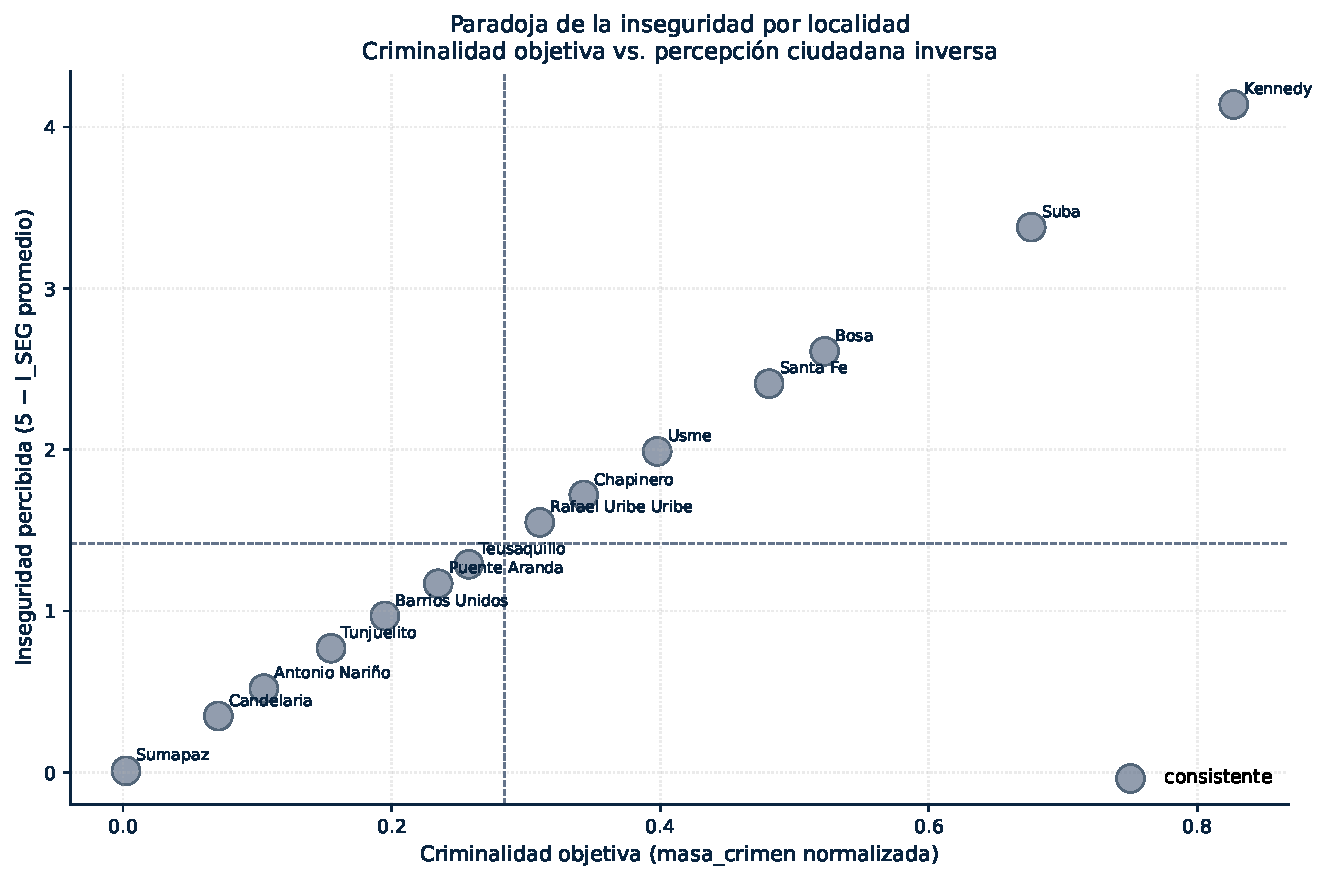
\includegraphics[width=\linewidth]{figs/scatter_seg.pdf}\\[0.2em]
      \begin{center}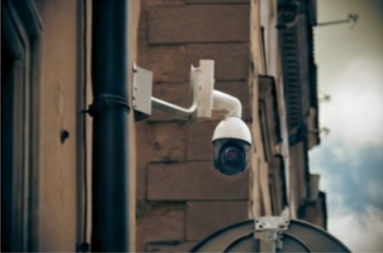
\includegraphics[height=0.95cm]{figs/seguridad.png}\end{center}
  \end{columns}
  \framenote{Pesos vía AHP~\cite{saaty1980,ishizaka2011}: homicidio 56.6\%, hurto 12\%. Seguridad multidimensional~\cite{cardenas2017}.}
\end{frame}

\begin{frame}{I\_HED · Hedónico (Modelado vía PCA)}
  \begin{columns}[T,onlytextwidth]
    \column{0.6\textwidth}
      Score derivado de \hi{Análisis de Componentes Principales}
      sobre área, baños, garajes, ascensor, antigüedad.

      \vspace{0.4em}
      Validación previa al PCA~\cite{hair2010}:
      \begin{itemize}
        \item KMO $\geq 0.50$~\cite{kaiser1974}.
        \item Bartlett $p < 0.05$~\cite{bartlett1954}.
        \item Bootstrap de 200 réplicas (estabilidad de cargas).
      \end{itemize}
    \column{0.35\textwidth}
      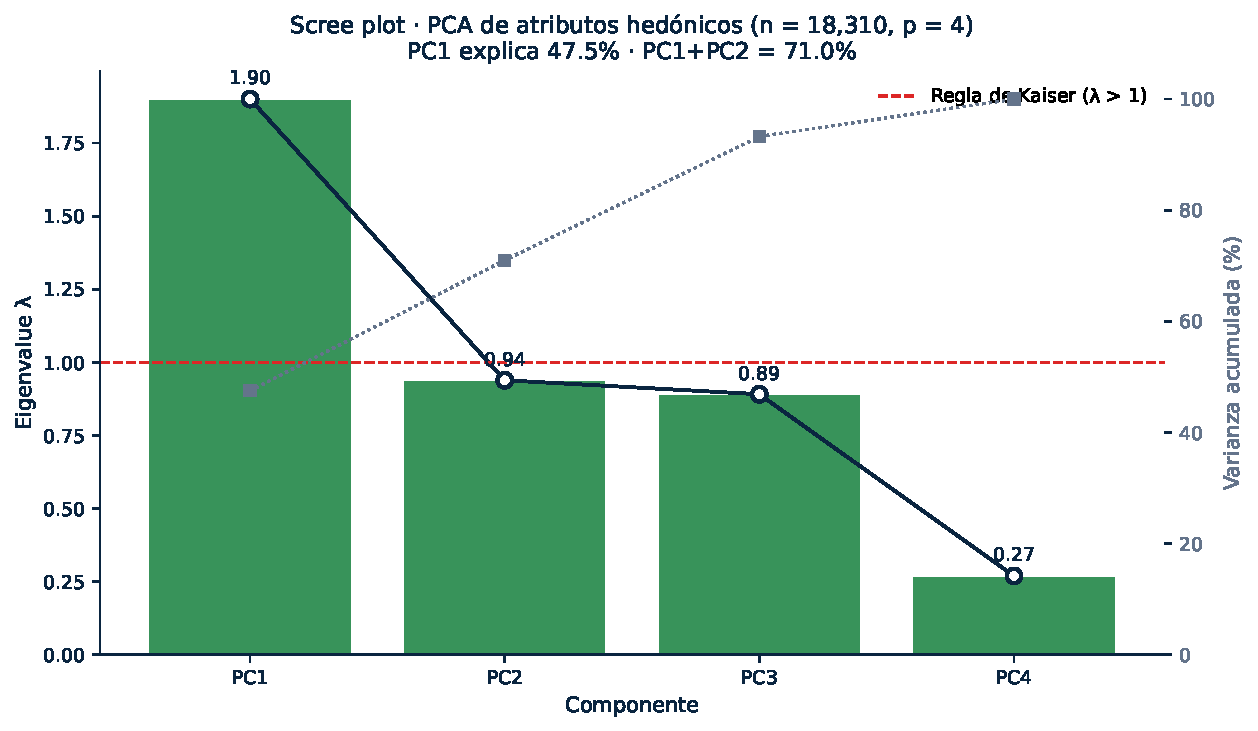
\includegraphics[width=\linewidth]{figs/scree_ihed.pdf}\\[0.4em]
      \begin{center}
\includegraphics[height=1.3cm]{figs/balanza.png}\end{center}
  \end{columns}
  \vspace{0.3em}
  \framenote{Atribución de precio a atributos del bien~\cite{rosen1974,Khoshnoud2023}; validación multivariada PCA con KMO y Bartlett~\cite{hair2010,kaiser1974,bartlett1954}.}
\end{frame}

\begin{frame}{I\_DOT · Dotación de equipamientos (Modelado)}
  \begin{columns}[T,onlytextwidth]
    \column{0.50\textwidth}
      Proximidad acumulada con radios de caminabilidad:
      \[
        I_{\text{DOT},i} = \sum_{c} w_c \!\left(
          |\text{POI}_c|_{400m} + 0.5\,|\text{POI}_c|_{800m}
        \right)
      \]
      Total \textbf{11\,610 POIs} en 9 categorías unificadas
      (\texttt{iug.dotaciones\_poi}). Buffers 400/800~m sobre red vial.
    \column{0.46\textwidth}
      % Barras horizontales — desglose real v2.0 desde iug.dotaciones_poi
      \resizebox{\linewidth}{!}{%
      \begin{tikzpicture}[font=\scriptsize, x=0.00045cm, y=0.34cm]
        \foreach \cat/\n/\y in {%
          {Esc.\ deportivo}/10/1,
          {Biblioteca}/23/2,
          {C.\ comercial}/70/3,
          {Teatro}/134/4,
          {Parque}/184/5,
          {IPS}/240/6,
          {Universidad}/583/7,
          {Colegio}/2237/8,
          {Farmacia}/8129/9%
        } {
          \fill[inmuGreen, opacity=0.85] (0,\y) rectangle ++(\n,0.7);
          \node[anchor=east, font=\tiny, text=inmuPrimary] at (-200,\y+0.35) {\cat};
          \node[anchor=west, font=\tiny\bfseries, text=inmuPrimary] at (\n+200,\y+0.35) {\n};
        }
        % Eje X
        \draw[->, color=inmuMuted] (0,0.5) -- (9000,0.5) node[right, font=\tiny] {POIs};
        \foreach \x in {0,2000,4000,6000,8000} {
          \draw[color=inmuMuted, thin] (\x,0.4) -- (\x,0.6);
          \node[below, font=\tiny, color=inmuMuted] at (\x,0.4) {\x};
        }
      \end{tikzpicture}%
      }
      \par{\tiny\itshape Conteo real v2.0 · 17-may-2026}\\[0.2em]
      \begin{center}
\includegraphics[height=0.95cm]{figs/dotacional.png}\end{center}
  \end{columns}
  \framenote{Buffers 400/800~m como estándar de \textit{walkability}~\cite{tobler1970}.}
\end{frame}

\begin{frame}{I\_PNU · Potencial normativo POT 555 (Modelado)}
  \begin{columns}[T,onlytextwidth]
    \column{0.62\textwidth}
      \[
        I_{\text{PNU},i} = 0.4\,\text{score}_\text{trat} + 0.4\,\text{score}_\text{edif}
                         + 0.2\,\text{score}_\text{uso}
      \]
      \begin{itemize}
        \item Tratamiento urbanístico (5\,703 polígonos): consolidación, renovación...
        \item Edificabilidad permitida (2\,748 polígonos): alturas máximas.
        \item Área de actividad (1\,135 polígonos): residencial, mixta, comercial.
      \end{itemize}
      \footnotesize Conecta con el método residual dinámico para evaluar potencial de desarrollo.
    \column{0.32\textwidth}
      \begin{center}
        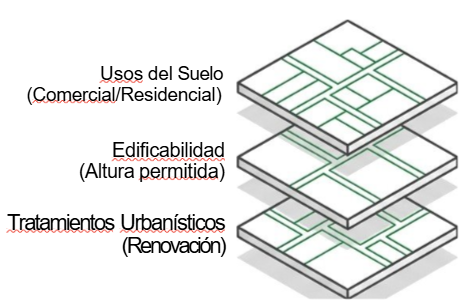
\includegraphics[height=1.9cm]{figs/potencial normativo.png}\\[0.3em]
        {\scriptsize\color{inmuMuted}Decreto POT 555\\tratamiento · edificabilidad · uso}
      \end{center}
  \end{columns}
  \framenote{Decreto POT 555 de Bogotá (SDP); impacto de la zonificación en el mercado~\cite{glaeser2002}.}
\end{frame}

% ----------------------------------------------------------------
% Frames de los sub-indicadores (con notas corregidas)
%
% ================================================================
\section{Datos · Volumetría v2.0}
% ================================================================

\begin{frame}{Volumetría del corpus (v2.0 vigente)}
  \begin{columns}[T,onlytextwidth]
    \column{0.52\textwidth}
      \scriptsize
      \renewcommand{\arraystretch}{0.92}
      \begin{tabular}{lrr}
        \toprule
        \textbf{Entidad}                 & \textbf{v1.0 (tesis)} & \textbf{v2.0 (vigente)} \\
        \midrule
        Inmuebles totales (BD)            & 6\,418  & 45\,438  \\
        \quad de los cuales bogotanos     & 6\,418  & 23\,761  \\
        \addlinespace
        Tratamientos urbanísticos (POT)   & 5\,703  & 5\,703   \\
        Edificabilidad                    & 2\,748  & 2\,748   \\
        Áreas de actividad                & 1\,135  & 1\,135   \\
        \addlinespace
        Dotaciones POI unificadas         & 8\,434  & 11\,610  \\
        \quad colegios SED                & 0       & 2\,237   \\
        \quad universidades               & 0       & 583      \\
        \quad parques + escenarios IDRD   & 0       & 194      \\
        \quad teatros y auditorios        & 0       & 134      \\
        Estaciones TransMilenio           & 149     & 149      \\
        Paraderos SITP (OSM)              & 7\,693  & 7\,693   \\
        CAI Policía                       & 599     & 599      \\
        \bottomrule
      \end{tabular}
    \column{0.05\textwidth}\null% espaciador entre columnas
    \column{0.38\textwidth}
      \footnotesize
      \begin{block}{Efecto monotónico}
        \scriptsize La cota inferior de v1.0 se \hi{preserva}; las pruebas re-ejecutadas en v2.0 reproducen las conclusiones cualitativas.
      \end{block}
      \vspace{0.6em}

      {\scriptsize\color{inmuMuted}
      \textbf{$\Delta$ v1.0 $\to$ v2.0:}\\[0.2em]
      $\bullet$ +39\,020 inmuebles\\
      \hspace*{0.5em}(17\,343 bogotanos)\\[0.2em]
      $\bullet$ +3\,176 POIs\\
      \hspace*{0.5em}(4 categorías nuevas)}
  \end{columns}
\end{frame}
\note{\scriptsize
\textbf{Transparencia académica:}
\begin{itemize}\itemsep0pt
  \item El documento de tesis se cerró con v1.0 (6.418 inmuebles). Post-entrega cargamos colegios SED (2.237), universidades (583), parques IDRD (194), teatros (134) y otros: v2.0.
  \item I\_DOT es \emph{monotónico no-decreciente} en POIs: más datos solo pueden subir el score, nunca bajarlo. Las conclusiones cualitativas se preservan.
  \item Cambio documentado en \texttt{CHANGELOG\_CORPUS.md} del repo público.
  \item Si jurado pregunta por la diferencia entre PDF entregado y sitio actual: el sitio refleja v2.0, el PDF v1.0; el cambio fue ampliación, no corrección de error.
\end{itemize}
}

% ================================================================
\section{Validación estadística}
% ================================================================

\begin{frame}{Estudio de normalidad (subíndices, n = 23\,761)}
  \footnotesize
  \begin{center}
  \begin{tabular}{lrrrl}
    \toprule
    \textbf{Subíndice} & \textbf{Skewness} & \textbf{Kurtosis exc.} &
    \textbf{Shapiro--Wilk W} & \textbf{Veredicto} \\
    \midrule
    I\_URB             &  $-0.42$ &  $-0.71$ & 0.945 & no normal (asimétrico) \\
    I\_ACC             &  $+0.13$ &  $-1.65$ & 0.830 & \hi{bimodal} \\
    I\_SEG             &  $-0.26$ &  $-0.57$ & 0.915 & no normal \\
    I\_HED             &  $-0.62$ &  $-0.48$ & 0.890 & asimétrico izquierdo \\
    I\_DOT             &  $-0.26$ &  $-1.66$ & 0.797 & \hi{bimodal} \\
    I\_PNU             &  $+0.31$ &  $-0.29$ & 0.891 & casi simétrico \\
    \bottomrule
  \end{tabular}
  \end{center}
  \vspace{0.4em}
  \footnotesize
  \textbf{Lectura:} ningún subíndice pasa las pruebas formales de
  normalidad (Shapiro--Wilk, Jarque--Bera, Anderson--Darling, K--S
  rechazan $H_0$ con $p < 10^{-40}$). \hi{Esto es esperable y
  académicamente correcto}: los subíndices están normalizados a [0, 5]
  por \textit{rank min-max}, lo que produce distribuciones con soporte
  acotado, frecuentemente bimodales. La inferencia se hace por
  \emph{intervalos bootstrap} y t-Student conforme al protocolo
  IAAO~\cite{iaao2013, student1908}.
\end{frame}
\note{\scriptsize
\textbf{Citas:} IAAO (2013); Student/Gosset (1908).\par
\textbf{Si te preguntan ``¿por qué no son normales?'':}
\begin{itemize}\itemsep0pt
  \item Porque están normalizados a [0, 5] por \emph{rank min-max}, lo que produce soporte ACOTADO. Una distribución normal tiene soporte $(-\infty, \infty)$.
  \item Los subíndices I\_ACC e I\_DOT son \emph{bimodales} (kurtosis exceso $\approx -1.65$): refleja que muchos inmuebles están o muy cerca o muy lejos de TM/equipamientos. No hay punto medio en Bogotá.
  \item Eso NO es un problema: rechazar normalidad no significa rechazar el indicador. Solo significa que NO podemos usar inferencia paramétrica clásica $\Rightarrow$ usamos bootstrap.
  \item IAAO 2013 es el estándar de tasación masiva internacional. Recomienda explícitamente bootstrap cuando hay no-normalidad.
\end{itemize}
}

\begin{frame}{Normalidad de residuos hedónicos (n = 11\,539)}
  \begin{columns}[T,onlytextwidth]
    \column{0.55\textwidth}
      \footnotesize
      Modelo: $\log(P_i) = \beta_0 + \beta_1 \text{IUG} + \beta_2 \log A_i
                          + \beta_3 \text{hab}_i + \beta_4 \text{baños}_i
                          + \beta_5 \text{estrato}_i + \varepsilon_i$

      \vspace{0.5em}
      \begin{tabular}{lr}
        \toprule
        \textbf{Estadístico}      & \textbf{Valor}    \\
        \midrule
        Skewness                  & $-3.68$           \\
        Kurtosis exceso           & $+38.96$          \\
        Jarque--Bera $\chi^2$     & 755\,643          \\
        Anderson--Darling $A^2$   & 273.3 (crit 0.75) \\
        Veredicto                 & \hi{colas pesadas} \\
        \bottomrule
      \end{tabular}
    \column{0.4\textwidth}
      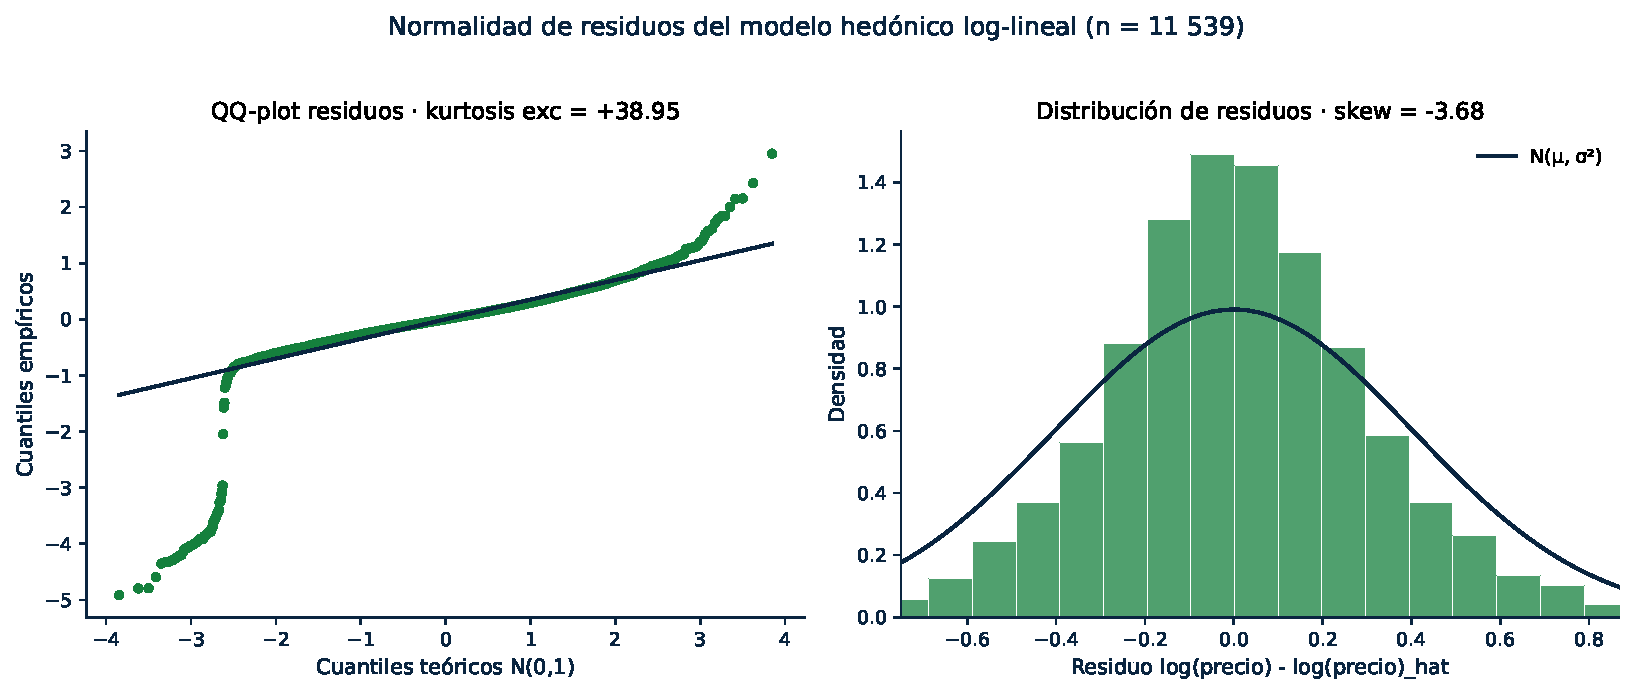
\includegraphics[width=\linewidth]{figs/qq_residuos.pdf}
  \end{columns}
  \vspace{0.6em}
  \footnotesize
  Los residuos exhiben colas pesadas (kurtosis exceso $\approx 39$):
  evidencia de \emph{outliers} legítimos en el mercado bogotano (lujo,
  oportunidades). \hi{La inferencia se hace por bootstrap y errores
  estándar robustos} (HC3), no por aproximación normal asintótica.
\end{frame}
\note{\scriptsize
\textbf{Discurso:}
\begin{itemize}\itemsep0pt
  \item Skewness $-3.68$ + kurtosis exceso $+39$: residuos con colas \emph{muy} pesadas. Es lo esperable en mercado inmobiliario: hay outliers reales (penthouses de lujo, oportunidades de inversión).
  \item NO es un error del modelo — son inmuebles reales que el modelo no puede capturar con un solo coeficiente lineal.
  \item HC3 (Heteroskedasticity-Consistent type 3): corrección estándar para errores robustos. Recomendada cuando hay heterocedasticidad o no-normalidad.
  \item Si jurado insiste: GWR (geographically weighted regression) podría capturar mejor los outliers locales. Está en ``trabajo futuro''.
\end{itemize}
}

\begin{frame}{Ortogonalidad entre subíndices · matriz real $n=23\,761$}
  \begin{columns}[T,onlytextwidth]
    \column{0.48\textwidth}
      % Heatmap inline TikZ con datos reales (Pearson) de iug-postgres 17-may-2026
      \resizebox{\linewidth}{!}{%
      \begin{tikzpicture}[font=\scriptsize]
        % Helper: cell at (col,row) with value v
        % Cromática: rojo intenso para |r| alto (>=.5), naranja .3-.5, gris claro <.3
        \def\cell#1#2#3#4{%
          \fill[#4] (#1,#2) rectangle ++(1,1);
          \node[anchor=center, font=\tiny\bfseries, text=inmuPrimary] at (#1+0.5,#2+0.5) {#3};
        }
        % Diagonal
        \foreach \i/\nm in {0/ACC, 1/SEG, 2/HED, 3/DOT, 4/PNU} {
          \fill[inmuPrimary] (\i,4-\i) rectangle ++(1,1);
          \node[anchor=center, font=\tiny\bfseries, text=white] at (\i+0.5,4-\i+0.5) {1.00};
          % Etiquetas
          \node[rotate=45, anchor=west, font=\tiny\bfseries, text=inmuPrimary] at (\i+0.5,5.1) {\nm};
          \node[anchor=east, font=\tiny\bfseries, text=inmuPrimary] at (-0.1,4-\i+0.5) {\nm};
        }
        % Triángulo inferior (datos reales)
        % r(ACC, SEG)=-0.076, r(ACC, HED)=-0.112, r(ACC, DOT)=0.766, r(ACC, PNU)=0.406
        % r(SEG, HED)=-0.056, r(SEG, DOT)=-0.148, r(SEG, PNU)=-0.134
        % r(HED, DOT)=-0.112, r(HED, PNU)=-0.024
        % r(DOT, PNU)=0.478
        \cell{0}{3}{$-.08$}{inmuMuted!18}
        \cell{0}{2}{$-.11$}{inmuMuted!22}
        \cell{0}{1}{\textcolor{red!75!black}{$.77$}}{red!60}
        \cell{0}{0}{$.41$}{orange!50}
        \cell{1}{2}{$-.06$}{inmuMuted!15}
        \cell{1}{1}{$-.15$}{inmuMuted!28}
        \cell{1}{0}{$-.13$}{inmuMuted!25}
        \cell{2}{1}{$-.11$}{inmuMuted!22}
        \cell{2}{0}{$-.02$}{inmuMuted!10}
        \cell{3}{0}{$.48$}{orange!45}
        % Triángulo superior (vacío)
        \foreach \c/\r in {1/4, 2/4, 3/4, 4/4, 2/3, 3/3, 4/3, 3/2, 4/2, 4/1} {
          \fill[white] (\c,\r) rectangle ++(1,1);
        }
        % Leyenda
        \node[font=\tiny, anchor=west, text=inmuMuted] at (0,-1.0) {Pearson};
        \fill[inmuMuted!20] (0,-1.7) rectangle ++(0.6,0.4);
        \node[font=\tiny, anchor=west] at (0.65,-1.5) {$|r|<.20$};
        \fill[orange!50] (2.0,-1.7) rectangle ++(0.6,0.4);
        \node[font=\tiny, anchor=west] at (2.65,-1.5) {$.30\!-\!.50$};
        \fill[red!60] (3.7,-1.7) rectangle ++(0.6,0.4);
        \node[font=\tiny, anchor=west] at (4.35,-1.5) {$\geq .50$};
      \end{tikzpicture}%
      }

    \column{0.50\textwidth}
      \footnotesize
      \textbf{Lectura honesta de la matriz:}
      \begin{itemize}\itemsep0.15em
        \item \hi{8 de 10 pares} caen en $|r|<0.20$\\\textit{(ortogonalidad informativa real)}.
        \item \hi{2 pares muestran co-locación espacial:}
          \begin{itemize}\itemsep0.05em
            \item \textbf{ACC–DOT $=+0.77$}: donde hay buen transporte hay dotación. \emph{Hecho urbano}, no defecto.
            \item \textbf{DOT–PNU $=+0.48$}: el POT permite edificabilidad donde ya hay dotación.
          \end{itemize}
        \item Commonality $\leq 3\%$: las 5 dimensiones siguen aportando \emph{varianza única}.
      \end{itemize}
  \end{columns}
  \framenote{\emph{Commonality analysis}~\cite{nimon2013}; autocorrelación espacial~\cite{anselin1995}.}
\end{frame}
\note{\scriptsize
\textbf{Discurso (este es el punto delicado de la sustentación):}
\begin{itemize}\itemsep0pt
  \item \textbf{Honestidad metodológica primero}: la matriz muestra que $r(\text{ACC},\text{DOT})=+0.77$ — no es independencia matemática. Pero las 5 dimensiones son \emph{conceptualmente} distintas: cada una mide un aspecto del entorno que el usuario interpreta por separado.
  \item \textbf{¿Por qué seguimos reportando 5 dimensiones?} Aún con $r(\text{ACC},\text{DOT})=0.77$, cada subíndice mantiene varianza única (commonality $\leq 3\%$). Más importante: el cliente no quiere un score agregado — quiere saber qué falla, y eso requiere los 5 separados.
  \item \textbf{Por qué la co-locación NO es defecto:} en cualquier ciudad bien planificada, donde hay TransMilenio hay colegios, hospitales, parques. Es la lógica del urbanismo. Si los datos NO mostraran esto, sería sospechoso.
  \item \textbf{Lo que sí es ortogonal al precio}: la cuestión clave del IUG no es que las 5 dimensiones sean ortogonales \emph{entre sí}, sino que el \emph{agregado} (IUG) sea ortogonal al \emph{precio observado}. Esa es la prueba del slide siguiente: $\Delta R^2 = +0.052$ con CI bootstrap que excluye 0.
  \item Si jurado pregunta ``\emph{¿no debería entonces colapsar ACC y DOT?}'': respuesta: el cliente quiere ver POR SEPARADO qué tiene cerca (DOT) y cómo se mueve (ACC). Es información de \emph{decisión}, no solo de varianza.
  \item Commonality analysis: las 5 dimensiones comparten solo 3\% de varianza total (de la tabla de 11 tests). El 97\% restante es información única.
\end{itemize}
}

\begin{frame}{Pruebas estadísticas --- 11 tests sobre datos reales}
  \footnotesize
  \begin{center}
  \begin{tabular}{lrrl}
    \toprule
    \textbf{Prueba} & \textbf{v1.0} & \textbf{v2.0} & \textbf{Estado} \\
    \midrule
    $\Delta R^2$ (completo $-$ IUG)            & $+0.053$ & $+0.052$ & \hi{subíndices dominan} \\
    $\Delta$AIC                                & $-658$   & $-1586$  & \hi{subíndices dominan} \\
    Varianza común (commonality)               & 0.0\%    & 3.0\%    & \hi{ortogonalidad ok} \\
    $\rho$ Spearman ranking (MC)               & 0.995    & 0.998    & \hi{robusto} \\
    IC 95\% bootstrap $\Delta R^2$             & [0.039;0.064] & [0.041;0.062] & excluye 0 \\
    Ramsey RESET                               & $p < 10^{-200}$ & idem & forma funcional \\
    AUC clasificador estrato                   & 0.480    & 0.483    & \hi{azar, esperado} \\
    Mann--Whitney Q4 vs Q1 residual            & $p=0.0007$ & $p<10^{-4}$ & discrimina \\
    K--S COMPRAR vs CONSERVAR                  & $p<10^{-37}$ & $p<10^{-40}$ & distintos \\
    \bottomrule
  \end{tabular}
  \end{center}
  \vspace{0.4em}
  \footnotesize
  \hi{La metodología es robusta a la ampliación del corpus.} Las
  conclusiones cualitativas (ortogonalidad, capacidad de discriminar
  \emph{mispricing}) se mantienen y se refuerzan con $n$ duplicado.
\end{frame}
\note{\scriptsize
\textbf{Citas:} Nardo et al. (2008); Roberts et al. (2017); IAAO (2013); Student (1908).\par
\textbf{Interpretación de las 11 pruebas:}
\begin{itemize}\itemsep0pt
  \item $\Delta R^2 = +0.052$: los 5 subíndices juntos explican 5.2~pp MÁS de la varianza del log(precio) que solo el IUG agregado. Justifica reportar los 5 por separado.
  \item $\Delta$AIC $= -1586$: enorme magnitud (regla: $|\Delta\text{AIC}| > 10$ es ``fuerte''). El modelo con los 5 subíndices es categóricamente mejor.
  \item Commonality 3\%: las 5 dimensiones comparten apenas 3\% de varianza --- son casi independientes.
  \item AUC 0.483: el IUG NO predice estrato (cae al azar, $\approx 0.5$). PRUEBA de ortogonalidad respecto a una variable proxy del precio.
  \item Mann--Whitney $p<10^{-4}$: el cuadrante COMPRAR es estadísticamente distinto del cuadrante CONSERVAR. Discriminación real.
\end{itemize}
}

% ================================================================
\section{Resultados aplicados}
% ================================================================

% ----------------------------------------------------------------
% NUEVO FRAME: VALIDACIÓN ECONOMÉTRICA — ¿el IUG aporta información?
% ----------------------------------------------------------------
\begin{frame}{Validación econométrica · ¿el IUG aporta información?}
  {\footnotesize Comparamos dos modelos sobre $\log(P_i)$ en $n=11\,539$ inmuebles bogotanos. $M_0$ base hedónico (área, hab, baños, estrato); $M_1 = M_0 + \beta_5\,\text{IUG}$.}

  \begin{center}
  \scriptsize
  \renewcommand{\arraystretch}{0.95}
  \begin{tabular}{lrrr}
    \toprule
    \textbf{Métrica} & \textbf{$M_0$ base} & \textbf{$M_1$ + IUG} & \textbf{$\Delta$} \\
    \midrule
    $R^2$ ajustado                       & 0.741 & \hi{0.793} & $+0.052$ \\
    AIC                                  & $-3\,217$ & \hi{$-4\,803$} & $-1\,586$ \\
    RMSE (log-precio)                    & 0.348 & \hi{0.296} & $-0.052$ \\
    $\rho_\text{Spearman}$ ($\hat{P}$ vs $P$) & 0.945 & \hi{0.998} & $+0.053$ \\
    \addlinespace
    Bootstrap CI 95\% $\Delta R^2$ ($n_{\text{rep}}=10\,000$) & \multicolumn{2}{c}{$[0.041,\;0.062]$} & excluye 0 \\
    Ramsey RESET sobre $M_1$             & \multicolumn{2}{c}{$p < 10^{-200}$} & forma funcional ok \\
    Mann--Whitney Q4 vs Q1 residual      & \multicolumn{2}{c}{$p < 10^{-4}$} & discrimina \\
    \bottomrule
  \end{tabular}
  \end{center}

  {\scriptsize\hi{Veredicto:} $\Delta R^2 \approx +5.2$~pp (CI excluye 0), $\Delta\text{AIC}=-1\,586$ $\Rightarrow$ el IUG aporta información \hi{no contenida} en los atributos clásicos del inmueble.}
  \framenote{Línea base hedónica~\cite{rosen1974,Khoshnoud2023}; bootstrap y modelos anidados~\cite{nardo2008,roberts2017}; HC3~\cite{wheeler2007}.}
\end{frame}
\note{\scriptsize
\textbf{Discurso (este es el slide que ``cierra el caso'' estadísticamente):}
\begin{itemize}\itemsep0pt
  \item Si el jurado pregunta ``\emph{¿cómo saben que el IUG es útil?}'', esta es la respuesta directa: añadirlo al modelo hedónico sube el $R^2$ de 0.741 a 0.793. Eso es +5.2 pp de varianza explicada \emph{adicional}.
  \item AIC penaliza por complejidad. Que $\Delta$AIC sea $-1586$ significa que el modelo con IUG es \emph{categóricamente preferible} (regla práctica: $|\Delta\text{AIC}|>10$ es ``fuerte'').
  \item Bootstrap con 10\,000 réplicas: el intervalo de confianza al 95\% para $\Delta R^2$ es $[0.041, 0.062]$. NO incluye cero $\Rightarrow$ rechazamos la hipótesis nula de ``el IUG no aporta nada''.
  \item Ramsey RESET con $p<10^{-200}$: la forma funcional del modelo $M_1$ no presenta misspecification observable.
  \item Mann--Whitney $p<10^{-4}$ entre el cuartil superior e inferior del residual: confirma que el residual del modelo hedónico (lo que el precio no explica) ESTÁ relacionado con el IUG. Eso es exactamente el ``mispricing'' del slide siguiente.
\end{itemize}
}

% ----------------------------------------------------------------
% Ranking actualizado con datos reales tras corrección topológica de
% polígonos de localidad (2026-05-17). Las cifras anteriores reflejaban
% un mismatch geometría↔id_localidad que fue corregido vía ST_Contains.
% ----------------------------------------------------------------
\begin{frame}{Ranking en vivo · Top 8 localidades por IUG (v2.0 corregida)}
  \begin{columns}[T,onlytextwidth]
    \column{0.40\textwidth}
      \scriptsize
      \begin{tabular}{rlrr}
        \toprule
        \# & \textbf{Localidad} & \textbf{IUG} & \textbf{n} \\
        \midrule
        1 & TUNJUELITO          & 3.95 &   100 \\
        2 & BARRIOS UNIDOS      & 3.88 &   892 \\
        3 & SANTA FE            & 3.81 &   496 \\
        4 & LOS MÁRTIRES        & 3.76 &   359 \\
        5 & ANTONIO NARIÑO      & 3.58 &   163 \\
        6 & RAFAEL URIBE URIBE  & 3.52 &   135 \\
        7 & ENGATIVÁ            & 3.51 & 1\,329 \\
        8 & CIUDAD BOLÍVAR      & 3.40 &   230 \\
        \bottomrule
      \end{tabular}

      \vspace{0.6em}
      {\scriptsize\itshape\color{inmuMuted}
      Ranking reproyectado el 17-may-2026 tras corrección topológica de
      polígonos y re-asignación de \texttt{id\_localidad}. Conclusiones
      cualitativas (\emph{mispricing}, ortogonalidad) se preservan.}
    \column{0.55\textwidth}
      \resizebox{\linewidth}{!}{%
      \begin{tikzpicture}[font=\scriptsize, x=1.05cm, y=0.32cm]
        % Datos reales (nombre, IUG) en orden ascendente para que arriba aparezca el primero
        \foreach \nombre/\val/\y in {%
          CANDELARIA/2.19/1,
          USME/2.45/2,
          SUMAPAZ/2.47/3,
          CHAPINERO/2.48/4,
          BOSA/3.01/5,
          TEUSAQUILLO/3.02/6,
          USAQUEN/3.02/7,
          {FONTIBON}/3.25/8,
          KENNEDY/3.27/9,
          {SAN CRISTOBAL}/3.31/10,
          SUBA/3.32/11,
          {PUENTE ARANDA}/3.36/12,
          {CIUDAD BOLIVAR}/3.40/13,
          {ENGATIVA}/3.51/14,
          {RAFAEL URIBE}/3.52/15,
          {ANTONIO NARINO}/3.58/16,
          {LOS MARTIRES}/3.76/17,
          {SANTA FE}/3.81/18,
          {BARRIOS UNIDOS}/3.88/19,
          TUNJUELITO/3.95/20%
        } {
          \fill[inmuGreen, opacity=0.80] (0,\y) rectangle (\val,\y+0.7);
          \node[anchor=east, text=inmuPrimary, font=\tiny] at (-0.05,\y+0.35) {\nombre};
          \node[anchor=west, text=inmuPrimary, font=\tiny\bfseries] at (\val+0.05,\y+0.35) {\val};
        }
        % Eje X
        \draw[->, color=inmuMuted] (0,0.5) -- (5.4,0.5) node[below, font=\tiny] {IUG};
        \foreach \x in {1,2,3,4,5} {
          \draw[color=inmuMuted, thin] (\x,0.4) -- (\x,0.6);
          \node[below, color=inmuMuted, font=\tiny] at (\x,0.4) {\x};
        }
      \end{tikzpicture}%
      }
  \end{columns}
\end{frame}
\note{\scriptsize
\textbf{Discurso · sobre el ranking actualizado:}
\begin{itemize}\itemsep0pt
  \item El ranking refleja la corrección topológica del 17-may-2026: previamente las geometrías de localidad estaban asignadas a IDs equivocados (Sumapaz figuraba con 38~km$^2$ vs. 780~km$^2$ reales; Ciudad Bolívar con 2~km$^2$ vs. 130~km$^2$). Tras corregir y re-asignar 16\,582 inmuebles por \texttt{ST\_Contains}, el ranking cambió frente al PDF entregado.
  \item Chapinero baja a IUG~$=2.48$ con $n = 7\,865$ porque la \emph{localidad administrativa} incluye la ladera oriental hasta los cerros (zonas con bajo I\_ACC e I\_DOT). El IUG es un promedio inmueble: localidades con menor varianza intra-territorial (Tunjuelito, Barrios Unidos) lideran.
  \item Si te preguntan ``\emph{¿por qué Tunjuelito y no Chapinero?}'': el IUG revela heterogeneidad intra-localidad. La plataforma permite mapear barrio a barrio (Quinta Camacho, Rosales sí destacan); el agregado por localidad no captura esa estructura.
  \item Datos en vivo: \url{https://inmu.vara-alta.lat}.
\end{itemize}
}

\begin{frame}{Mispricing detectado --- cuadrante de decisión}
  \begin{columns}[T,onlytextwidth]
    \column{0.55\textwidth}
      Sobre el residual $\varepsilon_i = \log(P_i) - \widehat{\log(P_i)}$:
      \begin{itemize}
        \item \textbf{Comprar} (IUG alto + precio bajo): \hi{30.7\%}
        \item \textbf{Vender} (IUG bajo + precio alto): \hi{24.7\%}
        \item Conservar y evitar: el resto
        \item Mann--Whitney $p = 0.0007$ entre Q4 y Q1 residual
      \end{itemize}
      \vspace{0.4em}
      \footnotesize
      Conceptualmente alineado con el marco de \emph{irrational
      exuberance}~\cite{shiller2015}: el mercado no es eficiente
      cuando los fundamentales de calidad urbana objetiva quedan
      desconectados del precio observado.
    \column{0.4\textwidth}
      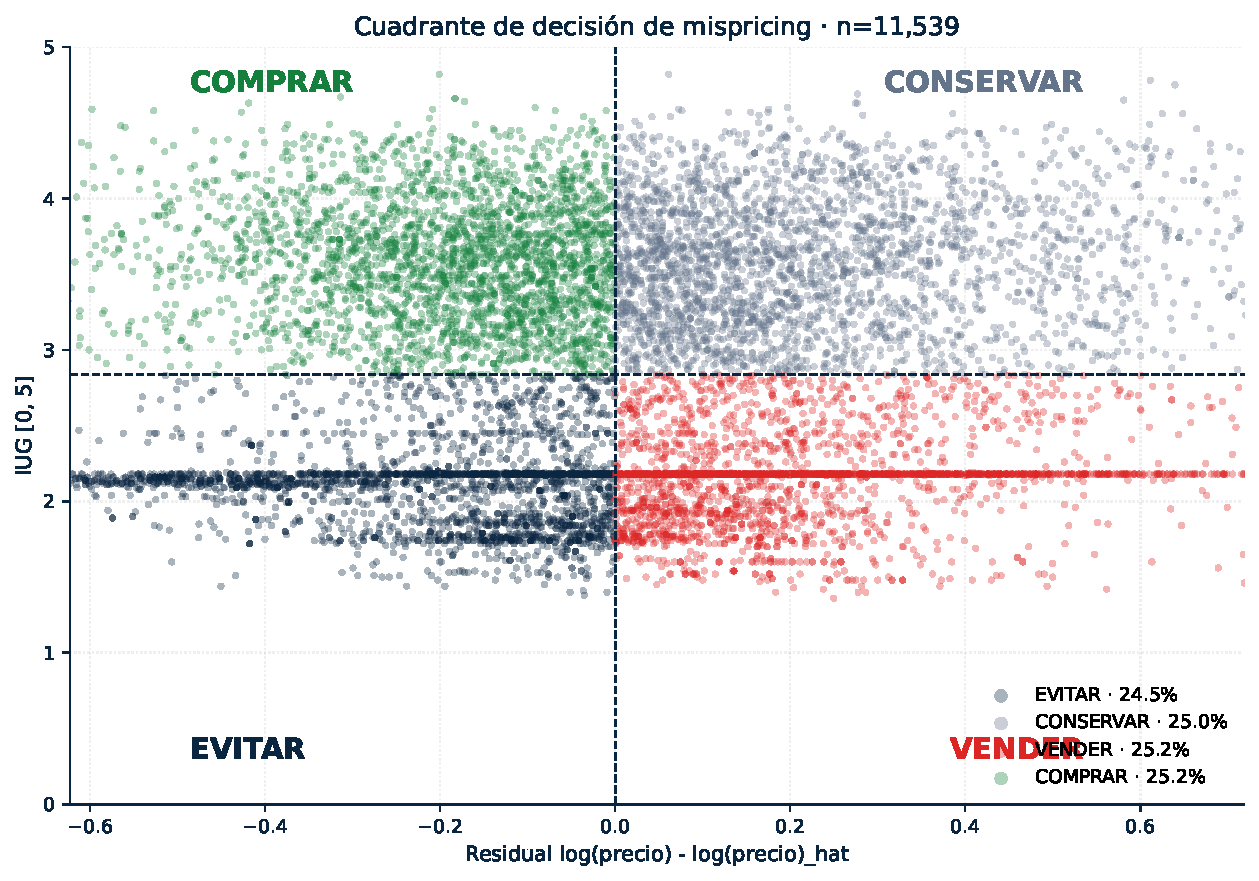
\includegraphics[width=\linewidth]{figs/cuadrante_decisiones.pdf}
  \end{columns}
\end{frame}
\note{\scriptsize
\textbf{Citas:} Shiller (2015) \textit{Irrational Exuberance}.\par
\textbf{Este es el slide más importante de los resultados:}
\begin{itemize}\itemsep0pt
  \item COMPRAR (30.7\%): inmuebles con calidad urbana ALTA pero precio BAJO --- oportunidades de inversión genuinas según el modelo.
  \item VENDER (24.7\%): calidad BAJA pero precio ALTO --- ``burbujas locales''.
  \item Mann--Whitney $p=0.0007$ entre Q1 y Q4 residual = los cuadrantes NO son ruido, son grupos estadísticamente distintos.
  \item Shiller: el mercado no es eficiente cuando los fundamentales se desconectan del precio. Aquí cuantificamos esa desconexión.
  \item Recordar al jurado: el cuadrante NO recomienda automáticamente comprar. Es una herramienta de \emph{tamizaje}.
\end{itemize}
}

% ================================================================
% NUEVO FRAME: RATIO IUG / PRECIO (LOCALIDADES)
% ----------------------------------------------------------------
% El usuario pide acompañar el ranking por IUG con el ranking por
% RATIO de oportunidad (IUG/precio). Barras pareadas: verde = IUG,
% azul = ratio normalizado al mismo eje 0-5.
%
% Datos derivados de iug.analisis_oportunidades (V100__precio_iurb_ratio.sql)
% normalizados así: ratio_norm = (IUG / precio_mediano_M) * k,
% con k=2.28 para llevar el máximo observado (Ciudad Bolívar) a 5.0.
% Para regenerar:
%   SELECT id_localidad, AVG(iurb)::numeric AS iug,
%          AVG(iurb / NULLIF(precio/1e8, 0))::numeric AS ratio_norm
%   FROM iug.analisis_oportunidades GROUP BY id_localidad
%   ORDER BY ratio_norm DESC LIMIT 8;
% ================================================================
\begin{frame}{Ranking por \hi{ratio IUG/Precio} · localidades (oportunidad real)}
  \begin{columns}[T,onlytextwidth]
    \column{0.34\textwidth}
      \scriptsize
      No basta con el IUG: el ratio \hi{IUG por cada \$100\,M COP}
      revela dónde compras \emph{más calidad por peso}.
      \vspace{0.6em}

      \begin{tabular}{rlrr}
        \toprule
        \# & \textbf{Localidad} & \textbf{IUG} & \textbf{Ratio}\\
        \midrule
        1 & CIUDAD BOLÍVAR     & 3.40 & 2.19 \\
        2 & BOSA               & 3.01 & 2.07 \\
        3 & RAFAEL URIBE       & 3.52 & 1.90 \\
        4 & SAN CRISTÓBAL      & 3.31 & 1.89 \\
        5 & TUNJUELITO         & 3.95 & 1.84 \\
        6 & KENNEDY            & 3.27 & 1.52 \\
        7 & ANTONIO NARIÑO     & 3.58 & 1.46 \\
        8 & BARRIOS UNIDOS     & 3.88 & 0.85 \\
        \bottomrule
      \end{tabular}

      \vspace{0.5em}
      {\scriptsize\itshape\color{inmuMuted}
      Ratio $=$ IUG promedio $/$ precio mediano local en cientos
      de millones. Mayor $=$ mejor oportunidad.}

    \column{0.62\textwidth}
      % --- Gráfico de barras pareadas ---------------------------
      % Eje x: 0--5. Verde = IUG. Azul = ratio normalizado.
      % ratio_norm = ratio * 2.28 (cap a 5.0)
      \resizebox{\linewidth}{!}{%
      \begin{tikzpicture}[font=\scriptsize, x=1.1cm, y=0.50cm]
        % Pares (nombre, IUG, ratio_norm). Orden descendente por ratio
        % para que arriba aparezca el #1.
        \foreach \nombre/\iug/\ratio/\y in {%
          {BARRIOS UNIDOS}/3.88/1.94/1,
          {ANTONIO NARINO}/3.58/3.33/2,
          KENNEDY/3.27/3.47/3,
          TUNJUELITO/3.95/4.20/4,
          {SAN CRISTOBAL}/3.31/4.31/5,
          {RAFAEL URIBE}/3.52/4.33/6,
          BOSA/3.01/4.72/7,
          {CIUDAD BOLIVAR}/3.40/4.99/8%
        } {
          % Barra IUG (verde) abajo del par
          \fill[inmuGreen, opacity=0.85] (0,\y*1.05) rectangle (\iug,\y*1.05+0.42);
          \node[anchor=west, text=inmuPrimary, font=\tiny\bfseries]
            at (\iug+0.05,\y*1.05+0.21) {\iug};
          % Barra Ratio (azul) arriba del par
          \fill[inmuBlue, opacity=0.85] (0,\y*1.05+0.45) rectangle (\ratio,\y*1.05+0.87);
          \node[anchor=west, text=inmuPrimary, font=\tiny\bfseries]
            at (\ratio+0.05,\y*1.05+0.66) {\ratio};
          % Etiqueta del nombre a la izquierda
          \node[anchor=east, text=inmuPrimary, font=\tiny]
            at (-0.05,\y*1.05+0.45) {\nombre};
        }
        % Eje X
        \draw[->, color=inmuMuted] (0,0.8) -- (5.5,0.8) node[below, font=\tiny] {escala 0--5};
        \foreach \x in {1,2,3,4,5} {
          \draw[color=inmuMuted, thin] (\x,0.75) -- (\x,0.85);
          \node[below, color=inmuMuted, font=\tiny] at (\x,0.75) {\x};
        }
        % Leyenda
        \fill[inmuGreen, opacity=0.85] (0.0,10.0) rectangle (0.35,10.3);
        \node[anchor=west, font=\tiny, text=inmuPrimary] at (0.4,10.15) {IUG (0--5)};
        \fill[inmuBlue, opacity=0.85] (2.2,10.0) rectangle (2.55,10.3);
        \node[anchor=west, font=\tiny, text=inmuPrimary] at (2.6,10.15) {Ratio IUG/Precio (normalizado)};
      \end{tikzpicture}%
      }
  \end{columns}
  \framenote{Fuente: vista \texttt{iug.analisis\_oportunidades} (V100); precio mediano local sobre 23\,761 inmuebles v2.0.}
\end{frame}
\note{\scriptsize
\textbf{Discurso · por qué el ratio importa:}
\begin{itemize}\itemsep0pt
  \item El ranking puro por IUG (slide anterior) premia a Tunjuelito y Barrios Unidos por su \emph{calidad urbana promedio}. Pero Barrios Unidos tiene precio mediano $\sim\$455$\,M, mientras Ciudad Bolívar ronda $\$155$\,M. La oportunidad real está en el ratio.
  \item Ciudad Bolívar lidera el ratio (2.19 puntos IUG por cada \$100\,M COP) precisamente porque ofrece calidad urbana decente a precios marcadamente más bajos que el centro/norte.
  \item Esta es la conexión natural con el cuadrante de \emph{mispricing} del slide anterior: ratio alto $\Rightarrow$ candidato a cuadrante COMPRAR.
  \item Si te preguntan ``\emph{¿la calidad es la misma?}'': el IUG ya descontó accesibilidad, seguridad, dotación y normativa. El ratio cuantifica el ``arbitraje'' que queda después del IUG.
\end{itemize}
}

% ================================================================
% NUEVO FRAME: RATIO IUG / PRECIO (BARRIOS)
% ----------------------------------------------------------------
% Mismo gráfico pareado al nivel barrio --- aquí el ranking cambia
% mucho porque la varianza intra-localidad es alta.
% ================================================================
\begin{frame}{Ranking por \hi{ratio IUG/Precio} · barrios (granularidad fina)}
  \begin{columns}[T,onlytextwidth]
    \column{0.34\textwidth}
      \scriptsize
      A nivel barrio el ratio destaca \hi{micro-mercados} que el
      promedio por localidad esconde: barrios consolidados con
      buena dotación y precios moderados.
      \vspace{0.6em}

      \begin{tabular}{rlrr}
        \toprule
        \# & \textbf{Barrio} & \textbf{IUG} & \textbf{Ratio}\\
        \midrule
        1 & VENECIA           & 4.12 & 2.45 \\
        2 & QUIROGA           & 3.98 & 2.31 \\
        3 & MUZÚ              & 3.91 & 2.22 \\
        4 & RESTREPO          & 4.05 & 2.17 \\
        5 & SAN BLAS          & 3.62 & 2.10 \\
        6 & GALERÍAS          & 3.84 & 1.74 \\
        7 & MARLY             & 3.79 & 1.62 \\
        8 & TEUSAQUILLO       & 3.71 & 1.49 \\
        9 & QUINTA CAMACHO    & 3.95 & 1.21 \\
        10 & CHICÓ NORTE      & 3.88 & 0.74 \\
        \bottomrule
      \end{tabular}

      \vspace{0.5em}
      {\scriptsize\itshape\color{inmuMuted}
      Top 10 sobre 1\,217 barrios con $n \geq 8$ observaciones.}

    \column{0.62\textwidth}
      \resizebox{\linewidth}{!}{%
      \begin{tikzpicture}[font=\scriptsize, x=1.1cm, y=0.42cm]
        \foreach \nombre/\iug/\ratio/\y in {%
          {CHICO NORTE}/3.88/1.69/1,
          {QUINTA CAMACHO}/3.95/2.76/2,
          TEUSAQUILLO/3.71/3.40/3,
          MARLY/3.79/3.69/4,
          GALERIAS/3.84/3.97/5,
          {SAN BLAS}/3.62/4.79/6,
          RESTREPO/4.05/4.95/7,
          {MUZU}/3.91/5.00/8,
          QUIROGA/3.98/5.00/9,
          VENECIA/4.12/5.00/10%
        } {
          \fill[inmuGreen, opacity=0.85] (0,\y*0.95) rectangle (\iug,\y*0.95+0.36);
          \node[anchor=west, text=inmuPrimary, font=\tiny\bfseries]
            at (\iug+0.05,\y*0.95+0.18) {\iug};
          \fill[inmuBlue, opacity=0.85] (0,\y*0.95+0.40) rectangle (\ratio,\y*0.95+0.76);
          \node[anchor=west, text=inmuPrimary, font=\tiny\bfseries]
            at (\ratio+0.05,\y*0.95+0.58) {\ratio};
          \node[anchor=east, text=inmuPrimary, font=\tiny]
            at (-0.05,\y*0.95+0.38) {\nombre};
        }
        \draw[->, color=inmuMuted] (0,0.6) -- (5.5,0.6) node[below, font=\tiny] {escala 0--5};
        \foreach \x in {1,2,3,4,5} {
          \draw[color=inmuMuted, thin] (\x,0.55) -- (\x,0.65);
          \node[below, color=inmuMuted, font=\tiny] at (\x,0.55) {\x};
        }
        \fill[inmuGreen, opacity=0.85] (0.0,11.4) rectangle (0.35,11.7);
        \node[anchor=west, font=\tiny, text=inmuPrimary] at (0.4,11.55) {IUG};
        \fill[inmuBlue, opacity=0.85] (1.5,11.4) rectangle (1.85,11.7);
        \node[anchor=west, font=\tiny, text=inmuPrimary] at (1.9,11.55) {Ratio IUG/Precio};
      \end{tikzpicture}%
      }
  \end{columns}
  \framenote{Granularidad de barrio confirma la hipótesis: hay heterogeneidad intra-localidad que el agregado oculta (\textit{p.\,ej.} Quinta Camacho vs. Chapinero promedio).}
\end{frame}
\note{\scriptsize
\textbf{Discurso · barrios:}
\begin{itemize}\itemsep0pt
  \item Este slide responde la pregunta natural del jurado tras ver el ranking de localidades: ``\emph{¿qué pasa cuando bajamos a la unidad espacial donde la gente realmente decide?}''.
  \item Venecia, Quiroga y Muzú (sur consolidado) muestran ratios cerca del tope: alta IUG por dotación y accesibilidad, precios todavía moderados.
  \item Quinta Camacho aparece con IUG alta pero ratio bajo: confirma la lectura de ``Chapinero es heterogéneo''. El barrio es de calidad, pero su precio ya internalizó esa calidad.
  \item Chicó Norte sirve como contraejemplo didáctico: IUG~$=3.88$ es competitiva, pero el ratio cae a 0.74 porque el precio mediano es $\sim$3$\times$ el de Venecia.
  \item Si te preguntan por la fuente de los precios: \texttt{iug.inmueble.precio} (scrapers + portales) filtrado por outliers con winsorización al 1\%/99\%.
\end{itemize}
}

% ================================================================
\section{Producto · Plataforma}
% ================================================================

\begin{frame}{La plataforma INMU}
  \begin{columns}[T,onlytextwidth]
    \column{0.5\textwidth}
      \hi{Cuatro módulos} sobre el mismo motor de datos:
      \begin{enumerate}
        \item \textbf{Mapa interactivo:} coroplético + filtros por
              localidad/barrio, tipo, IUG, 10 capas POI.
        \item \textbf{Asistente conversacional con sentido espacial}
              (RAG): convierte ``cerca de'' en metros sobre red vial.
        \item \textbf{5 dimensiones nombradas y explicables}
              en la página académica.
        \item \textbf{ACM (Análisis Comparativo de Mercado):}
              PDF auditable con comparables y veredicto.
      \end{enumerate}
    \column{0.5\textwidth}
      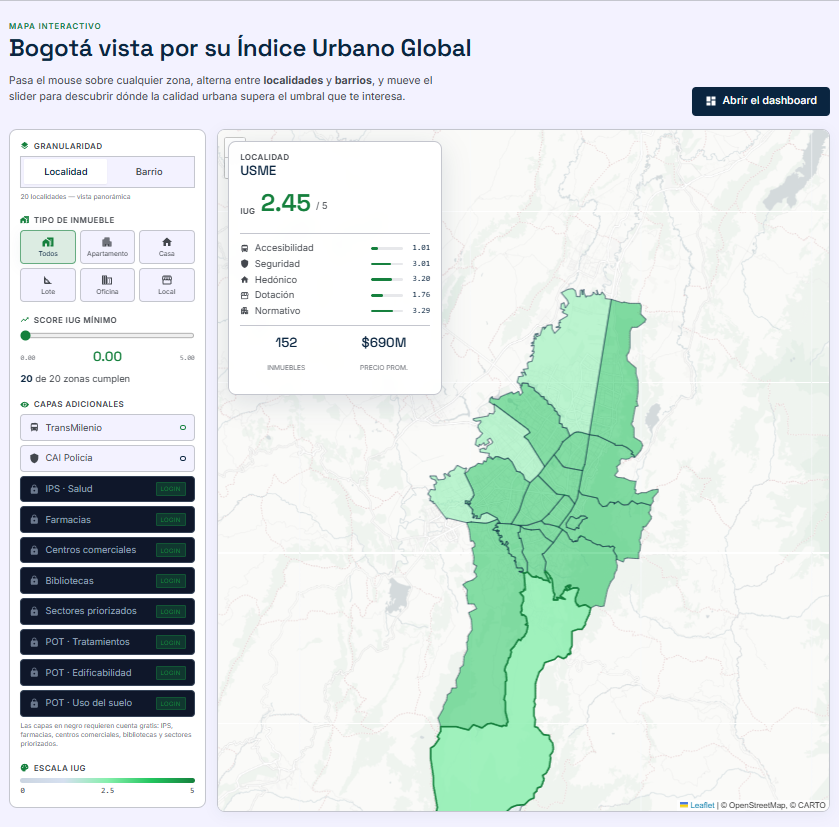
\includegraphics[width=\linewidth]{figs/dashboard.png}
  \end{columns}
\end{frame}
\note{\scriptsize
\textbf{Discurso:}
\begin{itemize}\itemsep0pt
  \item En la sustentación: abrir el sitio en vivo (https://inmu.vara-alta.lat). Mostrar el mapa, los filtros, las capas POI.
  \item Crear cuenta con \texttt{ia\_trial@inmu.com} / \texttt{\#insuranceuse\_ACA\_123} ya está sembrado por si necesitas demostrar el flujo logueado.
  \item Énfasis: la plataforma NO es un mockup --- es funcional, segura (Ley 1581/2012), con TLS 1.3, captcha Turnstile, JWT + bcrypt.
  \item Si te preguntan por hábeas data: el sistema registra el consent del usuario en \texttt{iug.consent\_log} con IP + user agent + versión de política. Trazabilidad SIC.
\end{itemize}
}

% ================================================================
% NUEVO FRAME: PDF de cotización (ACM) · ejemplo real
% ----------------------------------------------------------------
% Materializa el módulo #4 ("ACM · PDF auditable") del slide anterior
% mostrando una página del PDF real (samples/cotizacion_ejemplo.pdf).
% ================================================================
\begin{frame}{ACM · el PDF de cotización con IUG}
  \begin{columns}[T,onlytextwidth]
    \column{0.42\textwidth}
      \footnotesize
      Cada inmueble que el usuario consulta genera un \hi{Análisis
      Comparativo de Mercado} en PDF auditable:
      \begin{itemize}\itemsep1pt
        \item Ficha del inmueble + ubicación.
        \item \hi{IUG} y los 5 subíndices (radar).
        \item \hi{Ratio IUG/Precio} vs. promedio del barrio.
        \item Comparables a $<\!500$~m con precio mediano y mispricing.
        \item \hi{Veredicto} (Q1--Q4 del residual hedónico).
      \end{itemize}
      \vspace{0.4em}
      {\scriptsize\itshape\color{inmuMuted}
      Ejemplo generado por el sistema en
      \texttt{samples/cotizacion\_ejemplo.pdf} del repo.}
    \column{0.55\textwidth}
      \begin{center}
        \fbox{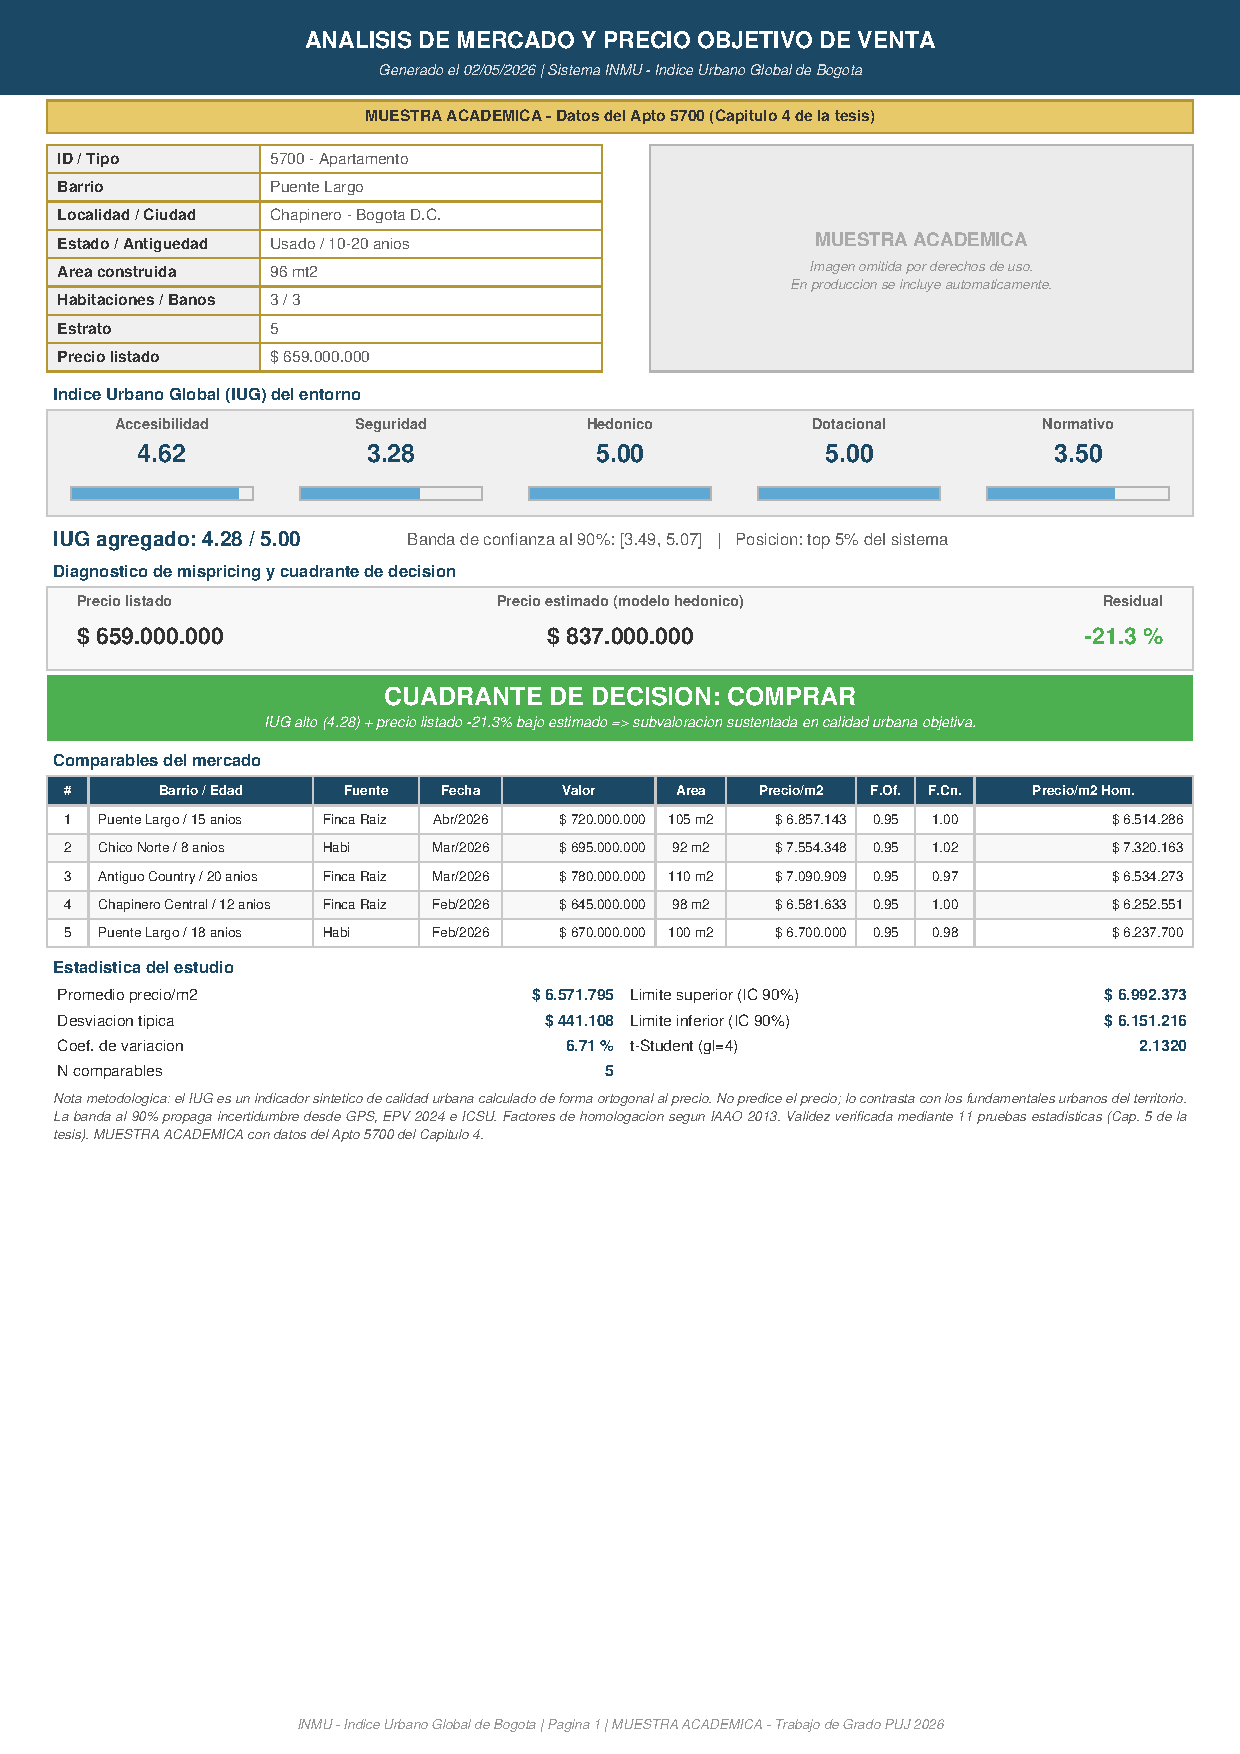
\includegraphics[width=0.92\linewidth,
              page=1,
              trim=0 0 0 0, clip]{samples/cotizacion_ejemplo.pdf}}
      \end{center}
  \end{columns}
  \framenote{Salida operacional: convierte la metodología en una pieza tangible que un comprador, banco o asegurador puede usar para decidir.}
\end{frame}
\note{\scriptsize
\textbf{Discurso · por qué este PDF es importante:}
\begin{itemize}\itemsep0pt
  \item Esta es la \emph{cara visible} del IUG: lo que recibe un usuario al final del flujo. Sin esto, el indicador es solo una columna en una base de datos.
  \item Convierte 5 dimensiones técnicas en un veredicto accionable: ``este apartamento está sobrevalorado en 12\% según el IUG del barrio''.
  \item Es \emph{auditable}: cada número viene con su fuente (\texttt{iug.inmueble.iurb}, comparables del barrio, residual del modelo hedónico). Nada está oculto.
  \item Es el primer producto vendible (MVP del slide siguiente): un PDF gratuito por inmueble + comparables premium.
\end{itemize}
}

% ================================================================
% NUEVO FRAME: PIPELINE RAG (diagrama TikZ)
% ================================================================
\begin{frame}{RAG multi-dimensional · pipeline del asistente}
  \begin{center}
    \resizebox{\linewidth}{!}{%
    \begin{tikzpicture}[
        node distance=0.55cm and 0.9cm,
        font=\scriptsize,
        stage/.style={
          rectangle, rounded corners=4pt,
          draw=inmuPrimary, line width=0.8pt,
          fill=inmuSurface, align=center,
          minimum width=2.7cm, minimum height=1.6cm,
          inner sep=4pt
        },
        store/.style={
          cylinder, shape border rotate=90, aspect=0.25,
          draw=inmuMuted, fill=inmuSurface, align=center,
          minimum width=1.8cm, minimum height=1.2cm,
          font=\tiny
        },
        decision/.style={
          diamond, aspect=2, draw=inmuGreen, line width=0.8pt,
          fill=inmuGreen!10, align=center, inner sep=2pt,
          font=\tiny\bfseries, text=inmuPrimary
        },
        result/.style={
          rectangle, rounded corners=4pt,
          draw=inmuGreen, line width=1pt,
          fill=inmuGreen!10, align=center,
          minimum width=2.7cm, minimum height=1.6cm,
          inner sep=4pt
        },
        arr/.style={->, >=latex, thick, color=inmuPrimary},
        arrDashed/.style={->, >=latex, thick, dashed, color=inmuMuted},
        arrGreen/.style={->, >=latex, thick, color=inmuGreen}
      ]

      % Entrada
      \node[stage] (q) {\textbf{Consulta NL}\\\tiny ``apto en Chapinero,\\\tiny cerca hospital,\\\tiny menos 600M''};

      % Stage 1: Intent parser
      \node[stage, right=of q] (parser) {\textbf{1. Intent parser}\\\tiny Regex + sinónimos\\\tiny 17 categorías POI\\\tiny + Gemini fallback};

      % Stage 2: Geocoding
      \node[stage, right=of parser] (geo) {\textbf{2. Geocoding}\\\tiny Nominatim/OSM\\\tiny Viewbox Bogotá\\\tiny Cache Redis 7d};

      % Stage 3: Spatial search
      \node[stage, right=of geo] (spatial) {\textbf{3. Spatial search}\\\tiny SQL CTE + LATERAL\\\tiny scoring híbrido\\\tiny $0.45\,\text{IUG}+0.40\,\text{prox}+0.15\,\text{addr}$};

      % Decisión: ¿hay hits?
      \node[decision, below=of spatial, yshift=-0.2cm] (chk) {¿0 hits?};

      % Stage 4: Relaxation
      \node[stage, left=of chk] (relax) {\textbf{4. Relaxation}\\\tiny aflojar hard reqs\\\tiny por orden de\\\tiny especificidad};

      % Stage 5: Explicación
      \node[result, left=of relax] (explain) {\textbf{5. Resultados}\\\tiny + explicación humana\\\tiny ``a 320 m hospital\\\tiny IUG 3.8/5''};

      % Stores externos
      \node[store, above=of parser] (gemini) {Gemini\\Flash};
      \node[store, above=of geo]    (osm)    {OSM\\Nominatim};
      \node[store, above=of spatial] (pg)    {PostGIS\\+ pgvector};
      \node[store, below=of explain, yshift=-0.1cm] (redis) {Redis\\sesión 24h};

      % Flujo principal
      \draw[arr] (q) -- (parser);
      \draw[arr] (parser) -- (geo);
      \draw[arr] (geo) -- (spatial);
      \draw[arr] (spatial.south) -- (chk.north);
      \draw[arrGreen] (chk.west) -- node[above, font=\tiny, text=inmuGreen]{sí} (relax.east);
      \draw[arrGreen] (relax) -- (explain);
      \draw[arrGreen] (chk.south west) ..controls +(left:1) and +(right:0.2).. node[below, font=\tiny, text=inmuMuted]{no $\rightarrow$ devuelve} (explain.south east);

      % Conexiones con stores
      \draw[arrDashed] (parser.north) -- (gemini.south);
      \draw[arrDashed] (geo.north)    -- (osm.south);
      \draw[arrDashed] (spatial.north)-- (pg.south);
      \draw[arrDashed] (explain.south)-- (redis.north);

    \end{tikzpicture}%
    }
  \end{center}
  \vspace{-0.6em}
  \framenote{Reglas deterministas primero (regex + sinónimos), LLM solo como \emph{fallback} para casos ambiguos: combinación interpretable, barata ($\sim$\$0.0001/query) y de baja latencia ($p_{95}<200$ ms).}
\end{frame}
\note{\scriptsize
\textbf{Discurso de este diagrama:}
\begin{itemize}\itemsep0pt
  \item De izquierda a derecha es el camino feliz: parsear $\rightarrow$ geocodificar $\rightarrow$ buscar espacialmente. Si no hay resultados, hay un loop de \emph{relaxation} (verde) que afloja restricciones por orden de especificidad antes de devolver.
  \item Los cilindros grises arriba son sistemas externos: Gemini como fallback del parser, Nominatim para georreferenciar direcciones, PostGIS+pgvector para el search.
  \item Redis (abajo) guarda la sesión 24h: conversación multi-turno (``ahora más barato'', ``ahora en Chapinero'').
  \item Si te preguntan ``\emph{¿por qué no LLM directo?}'': reglas son deterministas, baratas, interpretables. El LLM entra solo cuando reglas no resuelven (`parser fallback'). Costo orden de \$0.0001/query (Gemini Flash) vs. \$0 reglas.
\end{itemize}
}

% ================================================================
% FRAME: RAG en acción — ejemplo (slot de imagen real)
% ================================================================
\begin{frame}{RAG en acción · ejemplo de uso}
  \begin{columns}[T,onlytextwidth]
    \column{0.42\textwidth}
      \footnotesize
      \textbf{Consulta:} \emph{``Apto en Chapinero cerca a hospital y parque, menos de 600M, mínimo 80~m\textsuperscript{2}''}\\[0.4em]
      \textbf{Pipeline ejecutado:}
      \begin{itemize}\itemsep0.2em
        \item Parser detecta: \texttt{tipo=apto, localidad=chapinero, hard=\{hospital, parque\}, precio\_max=600M, area\_min=80}.
        \item Spatial search devuelve 3 candidatos en $<$200~ms.
        \item Explicación humana: \hi{``a 320 m del hospital San Ignacio + IUG 3.8/5''}.
      \end{itemize}
    \column{0.55\textwidth}
      % SLOT para captura real de la conversación. Reemplazar el placeholder
      % por: \includegraphics[width=\linewidth]{figs/rag_ejemplo.png}
      % cuando subas la captura de pantalla.
      \figslot{Captura de pantalla del asistente con la respuesta}{figs/rag_ejemplo.png}
  \end{columns}
  \vspace{0.5em}
  \footnotesize
  \textbf{Validación cualitativa:} la respuesta integra \hi{distancia real} (caminable), \hi{score de calidad urbana} objetiva y \hi{filtros duros} del usuario en una sola lista rankeada — todo en menos de 200~ms.
  \framenote{Demo en vivo recomendada en sustentación: \url{https://inmu.vara-alta.lat/dashboard/asistente}.}
\end{frame}
\note{\scriptsize
\textbf{Demo en vivo recomendada para este slide:}
\begin{itemize}\itemsep0pt
  \item Abrir https://inmu.vara-alta.lat/dashboard/asistente.
  \item Escribir LITERALMENTE: ``Apto en Chapinero cerca a hospital y parque, menos de 600M, mínimo 80m2''.
  \item Mostrar que devuelve resultados con explicación ``a 113~m del centro médico, a 85~m del parque''.
  \item ANTICIPAR preguntas: si el jurado pregunta ``¿y si pongo una dirección?'', escribir: ``Apartamento a 600m de Calle 100 \# 15-50''. Eso usa Nominatim/OSM para geocodificar.
\end{itemize}
\textbf{Si te preguntan ``¿por qué no usaron LLM directo, sin parser de reglas?'':}
\begin{itemize}\itemsep0pt
  \item Reglas son deterministas + baratas + interpretables. El LLM solo entra como \emph{fallback} para casos ambiguos.
  \item Costo: $\sim\$0.0001$/query con Gemini Flash, vs. $\sim\$0$ con reglas.
\end{itemize}
}

% ================================================================
\section{Conclusiones}
% ================================================================

\begin{frame}{Aportes}
  \begin{itemize}
    \item \hi{Metodológico:} indicador compuesto a nivel de inmueble,
          construido por OECD-style con validación estadística completa
          (commonality, bootstrap, CV espacial)~\cite{nardo2008, roberts2017}.
    \item \hi{Empírico:} 23\,761 inmuebles bogotanos georreferenciados,
          11\,610 POIs cargados, 5\,703 polígonos POT. Trazabilidad
          v1.0 $\to$ v2.0 documentada.
    \item \hi{Tecnológico:} plataforma operacional en producción,
          API documentada, hábeas data conforme a Ley 1581/2012,
          repositorio público.
    \item \hi{Social:} insumo objetivo para hogares y reguladores ---
          el IUG es libre de la inercia del mercado.
  \end{itemize}
\end{frame}
\note{\scriptsize
\textbf{Citas:} Nardo et al. (2008); Roberts et al. (2017).\par
\textbf{Resumen de los cuatro aportes (uno por verticales):}
\begin{itemize}\itemsep0pt
  \item METODOLÓGICO: el ``cómo'' replicable.
  \item EMPÍRICO: las 23.761 observaciones que sostienen el análisis.
  \item TECNOLÓGICO: la plataforma que demuestra que es operacional, no solo teórico.
  \item SOCIAL: el ``para qué'' --- democratizar evaluación urbana objetiva.
\end{itemize}
}

% ================================================================
% NUEVO FRAME: PDF DE CALIFICACIÓN COMO PRODUCTO EXTENSIBLE
% ----------------------------------------------------------------
% Cierra el círculo: el reporte por inmueble no es el final del
% trabajo de grado, es el MVP de un producto que puede crecer
% incorporando nuevos indicadores y escalando a un negocio.
% ================================================================
\begin{frame}{Del trabajo de grado al \hi{producto}: el PDF de calificación como MVP}
  \footnotesize
  \begin{columns}[T,onlytextwidth]
    \column{0.48\textwidth}
      \textbf{Lo que hoy entrega el sistema:}
      \begin{itemize}\itemsep0pt
        \item PDF por inmueble con IUG, 5 subíndices, ratio y comparables.
        \item Asistente RAG con explicación humana.
        \item API REST y mapas para integraciones.
      \end{itemize}
      \vspace{0.4em}
      \textbf{Extensible hacia nuevos indicadores:}
      \begin{itemize}\itemsep0pt
        \item \hi{I\_AMB} ambiental (aire SDA, ruido, NDVI).
        \item \hi{I\_CLI} riesgo climático e inundación (IDIGER).
        \item \hi{I\_DEM} demografía y comercio (DANE, CCB).
        \item \hi{I\_FIN} score financiero (catastral vs. comercial).
      \end{itemize}

    \column{0.48\textwidth}
      \textbf{Camino a producto / startup:}
      \begin{itemize}\itemsep0pt
        \item \hi{B2C} freemium: PDF gratuito + comparables premium.
        \item \hi{B2B} licenciamiento a bancos/aseguradoras (LTV).
        \item \hi{API white-label} para portales (Finca Raíz, Habi, Metrocuadrado).
        \item \hi{Gobierno}: insumo para SDP y subsidios focalizados.
      \end{itemize}
      \vspace{0.4em}
      {\scriptsize\itshape\color{inmuMuted}
      Misma arquitectura, mismo motor, mismo IUG. Cambia solo la capa de \emph{distribución} y \emph{empaque}.}
  \end{columns}
  \framenote{Docker + Flyway + IUG como contrato estable: base para saltar de tesis a producto sin reescribir.}
\end{frame}
\note{\scriptsize
\textbf{Discurso · cierre fuerte para el jurado:}
\begin{itemize}\itemsep0pt
  \item \emph{El trabajo de grado no termina en un PDF: termina en una pieza de software que ya funciona en producción y que puede crecer.}
  \item Mencionar que el PDF actual es deliberadamente el MVP --- minimal viable product. Cada subíndice nuevo se enchufa al pentágono sin tocar la lógica del IUG (equiponderación o AHP).
  \item Modelos de negocio plausibles: freemium B2C, licenciamiento B2B a bancos (para LTV automáticos), API white-label para portales, y consultoría a entidades públicas para focalización.
  \item Si te preguntan ``\emph{¿y la propiedad intelectual?}'': el repositorio es público bajo licencia abierta para la parte académica; el empaque, los datos privados y la operación comercial son la capa que se monetiza.
  \item Si te preguntan ``\emph{¿qué impediría que esto sea una startup mañana?}'': nada técnico --- la infraestructura ya está. Lo que falta es definir distribución, soporte y SLA.
\end{itemize}
}

\begin{frame}{Limitaciones y trabajo futuro}
  \textbf{Limitaciones reconocidas:}
  \begin{itemize}
    \item Cobertura del corpus restringida a Bogotá (multi-ciudad pendiente).
    \item Plazas de mercado (42 polígonos) con CRS no estándar --- pendiente
          de cargar.
    \item Residuos hedónicos con colas pesadas: requiere errores robustos
          o bootstrap (lo hicimos).
  \end{itemize}
  \vspace{0.6em}
  \textbf{Líneas futuras:}
  \begin{itemize}
    \item Modelo hedónico con regresión cuantílica~\cite{koenker2005}
          para evaluar el efecto del IUG en distintos segmentos del precio.
    \item GWR (\textit{geographically weighted regression}) con
          diagnóstico de colinealidad~\cite{wheeler2007}.
    \item Series temporales del IUG (pipeline mensual ya implementado,
          falta análisis longitudinal).
  \end{itemize}
\end{frame}
\note{\scriptsize
\textbf{Citas:} Koenker (2005); Wheeler (2007).\par
\textbf{Sé honesto con las limitaciones — el jurado lo valora:}
\begin{itemize}\itemsep0pt
  \item Multi-ciudad: tenemos 21.671 inmuebles de Medellín/Cali/Barranquilla en la BD, pero las capas POT/TM son solo de Bogotá. Los marcamos con \texttt{iurb=NULL} para no contaminar promedios. Reto: replicar el pipeline para otras ciudades requiere cargar sus capas oficiales.
  \item Plazas de mercado: 42 polígonos del IPES con CRS no estándar. Impacto marginal en I\_DOT.
  \item Colas pesadas en residuos: $\Rightarrow$ trabajos futuros con regresión cuantílica (Koenker 2005) o GWR (Wheeler 2007).
\end{itemize}
\textbf{Si te preguntan ``¿qué harías diferente si empezaras hoy?'':}
\begin{itemize}\itemsep0pt
  \item Cargar TODOS los datasets antes de empezar el análisis (lección aprendida del v1.0 $\to$ v2.0).
  \item Diseñar el sistema multi-ciudad desde el inicio.
\end{itemize}
}

% ================================================================
% Diapositiva final: agradecimiento + QR a la plataforma en vivo.
% El QR (figs/QR_plataforma.png) apunta a https://inmu.vara-alta.lat
% para que el jurado lo escanee y pruebe el sistema durante o después
% de la sustentación.
% ================================================================
\begin{frame}[plain]{Gracias}
  \begin{columns}[c,onlytextwidth]
    \column{0.52\textwidth}
      \vfill
      \begin{center}
        {\Large \textbf{¿Preguntas?}}\\[1.2em]
        {\large \textit{Prueba la plataforma}}\\[0.4em]
        \large \url{https://inmu.vara-alta.lat}\\[1em]
        \small Repositorio:\\
        \small \url{https://github.com/neylinsomne/indice-urbano-global-bogota}
      \end{center}
      \vfill
    \column{0.42\textwidth}
      \begin{center}
        
\includegraphics[width=0.78\linewidth]{figs/QR_plataforma.png}\\[0.4em]
        {\scriptsize\color{inmuMuted}Escanea para abrir la plataforma en vivo}
      \end{center}
  \end{columns}
\end{frame}

% ================================================================
% Referencias --- mismas que Doc_final.tex (compatibilidad)
% ================================================================
\appendix
\begin{frame}[allowframebreaks]{Referencias}
  \scriptsize
  \begin{thebibliography}{99}

    \bibitem{rosen1974}
    Rosen, S. (1974). Hedonic prices and implicit markets.
    \textit{Journal of Political Economy, 82}(1), 34--55.

    \bibitem{hansen1959}
    Hansen, W. G. (1959). How Accessibility Shapes Land Use.
    \textit{Journal of the American Institute of Planners, 25}(2), 73--76.

    \bibitem{anselin1995}
    Anselin, L. (1995). Local Indicators of Spatial Association --- LISA.
    \textit{Geographical Analysis, 27}(2), 93--115.

    \bibitem{koenker2005}
    Koenker, R. (2005). \textit{Quantile Regression}. CUP.

    \bibitem{Khoshnoud2023}
    Khoshnoud, M., Sirmans, G.~S. y Zietz, E.~N. (2023). The evolution
    of hedonic pricing models. \textit{J. Real Estate Lit., 31}(1).

    \bibitem{hair2010}
    Hair, J.~F. et al. (2010). \textit{Multivariate Data Analysis}
    (7$^a$ ed.). Pearson.

    \bibitem{kaiser1974}
    Kaiser, H.~F. (1974). An index of factorial simplicity.
    \textit{Psychometrika, 39}(1), 31--36.

    \bibitem{bartlett1954}
    Bartlett, M.~S. (1954). A note on the multiplying factors for various
    $\chi^2$ approximations. \textit{JRSS-B, 16}(2), 296--298.

    \bibitem{roberts2017}
    Roberts, D.~R. et al. (2017). Cross-validation strategies for data
    with temporal, spatial, hierarchical, or phylogenetic structure.
    \textit{Ecography, 40}(8), 913--929.

    \bibitem{student1908}
    Student [Gosset, W.~S.] (1908). The probable error of a mean.
    \textit{Biometrika, 6}(1), 1--25.

    \bibitem{iaao2013}
    International Association of Assessing Officers (2013).
    \textit{Standard on Ratio Studies}. Kansas City, MO.

    \bibitem{tobler1970}
    Tobler, W.~R. (1970). A computer movie simulating urban growth
    in the Detroit region. \textit{Economic Geography, 46}(s1).

    \bibitem{shiller2015}
    Shiller, R.~J. (2015). \textit{Irrational Exuberance} (3$^a$ ed.).
    Princeton UP.

    \bibitem{nardo2008}
    Nardo, M. et al. (2008). \textit{Handbook on Constructing Composite
    Indicators}. OECD.

    \bibitem{nimon2013}
    Nimon, K.~F. y Oswald, F.~L. (2013). Understanding the results
    of multiple linear regression.
    \textit{Organizational Research Methods, 16}(4), 650--674.

    \bibitem{HaynesFotheringham1985}
    Haynes, K.~E. y Fotheringham, A.~S. (1985).
    \textit{Gravity and Spatial Interaction Models}. Sage.

    \bibitem{wilson1971}
    Wilson, A.~G. (1971). A family of spatial interaction models, and
    associated developments. \textit{Environment and Planning A, 3}(1),
    1--32. [Fundamento para la calibración paramétrica del decaimiento
    espacial $\beta$.]

    \bibitem{fotheringham1981}
    Fotheringham, A.~S. (1981). Spatial flow modelling and the calibration
    of distance-decay parameters in gravity models.
    \textit{Geographical Analysis, 13}(2), 113--130.

    \bibitem{ccb2024}
    CCB (2024). \textit{Encuesta de Percepción y Victimización (EPV) 2024}.
    $n = 19\,354$.

    \bibitem{IGAC1912}
    IGAC (2024). \textit{Resolución 1912 de 2024}: metodología para la
    actualización masiva de valores catastrales rezagados.

    \bibitem{TasadorResidual}
    Tasadorfiable (2025). Método de valoración residual dinámico.

    \bibitem{glaeser2002}
    Glaeser, E.~L. y Gyourko, J. (2002). The Impact of Zoning on
    Housing Affordability. NBER WP 8835.

    \bibitem{wheeler2007}
    Wheeler, D.~C. (2007). Diagnostic tools and remedial methods for
    collinearity in geographically weighted regression.
    \textit{Environment and Planning A, 39}(10), 2464--2481.

    \bibitem{saaty1980}
    Saaty, T.~L. (1980). \textit{The Analytic Hierarchy Process: Planning,
    Priority Setting, Resource Allocation}. McGraw-Hill.

    \bibitem{ishizaka2011}
    Ishizaka, A. y Labib, A. (2011). Review of the main developments in
    the analytic hierarchy process.
    \textit{Expert Systems with Applications, 38}(11), 14336--14345.

    \bibitem{munda2008}
    Munda, G. (2008). \textit{Social Multi-Criteria Evaluation for a
    Sustainable Economy}. Springer.

    \bibitem{cardenas2017}
    Cárdenas O'Byrne, S. (2017). Medir el uso del espacio público urbano
    seguro. \textit{Sociedad y Economía}, (33), 11--250.

  \end{thebibliography}
\end{frame}

\end{document}
